% file thesis.tex
% Archivo thesis.tex
% Documento maestro que incluye todos los paquetes necesarios para el documento
% principal.

% Documento obtenido por un sinfin de iteraciones de administradores del LDC
% Estructura actual hecha por:
% Jairo Lopez <jairo@ldc.usb.ve>
% Actualizado ligeramente por:
% Alexander Tough 

\documentclass[oneside,12pt,letterpaper]{report}
\tolerance=1000  
\hbadness=10000  
\raggedbottom

% Para escribir algoritmos
\usepackage{listings}
\usepackage{algpseudocode}
\usepackage{algorithmicx}
\usepackage{algorithm}

% Paquetes para manejar graficos
\usepackage{epsf}
\usepackage[pdftex]{graphicx}
\usepackage{epsfig}
% Simbolos matematicos
\usepackage{latexsym,amssymb}
% Paquetes para presentar una tesis decente.
\usepackage{setspace,cite} % Doble espacio para texto, espacio singular para
                           % los caption y pie de pagina
\usepackage[table]{xcolor}
\usepackage{tikz}
\usepackage[T1]{fontenc}

\usetikzlibrary{shapes.geometric,arrows}

\usetikzlibrary{arrows,shapes}
\usepackage{verbatim}

\usepackage{comment}

% Paquetes no utilizados para citas
%\usepackage{mcite} 
%\usepackage{draft} 

\usepackage{wrapfig}
\usepackage{alltt}

% Acentos 
\usepackage[spanish,activeacute,es-noquoting]{babel}

\usepackage[spanish]{translator}
\usepackage[utf8]{inputenc}
\usepackage{color, xcolor, colortbl}
\usepackage{multirow}
\usepackage{subfig}
\usepackage[OT1]{fontenc}
\usepackage{tocbibind}
\usepackage{anysize}
\usepackage{listings} 

% Para poder tener texto asiatico
%\usepackage{CJK}

% Opciones para los glosarios
\usepackage[style=altlist,toc,numberline,acronym]{glossaries}
\usepackage{url}
\usepackage{amsthm}
\usepackage{amsmath}
\usepackage{fancyhdr} % Necesario para los encabezados
\usepackage{fancyvrb}
\usepackage{makeidx} % En caso de necesitar indices.
\makeindex  % Necesitado para los indices

% Definiciones para definicions, teoremas y lemas
\theoremstyle{definition} \newtheorem{definicion}{Definici\'{o}n}
\theoremstyle{plain} \newtheorem{teorema}{Teorema}
\theoremstyle{plain} \newtheorem{lema}{Lema}

% Para la creacion de los pdfs
\usepackage{hyperref}

% Para resolver el lio del Unicode para la informacion de los PDFs
% En pdftitle coloca el nombre de su proyecto de grado/pasantia.
% En pdfauthor coloca su nombre.
\hypersetup{
    pdftitle = {Desarrollo de un prototipo de robot humanoide que busque, encuentre y patee una pelota },
    pdfauthor={Jennifer Dos Reis y Juliana Leon},
    colorlinks,
    citecolor=black,
    filecolor=black,
    linkcolor=black,
    urlcolor=black,
    backref,
    pdftex
}

\definecolor{brown}{rgb}{0.7,0.2,0}
\definecolor{darkgreen}{rgb}{0,0.6,0.1}
\definecolor{darkgrey}{rgb}{0.4,0.4,0.4}
\definecolor{lightgrey}{rgb}{0.95,0.95,0.95}

\usepackage{listings}
\lstnewenvironment{code}{\lstset{basicstyle=\small}}{}

\lstset{escapeinside=~~}
\lstset{
   frame=single,
   framerule=1pt,
   showstringspaces=false,
   basicstyle=\footnotesize\ttfamily,
   keywordstyle=\textbf,
   backgroundcolor=\color{lightgrey}
}

% Crea el glosario
\makeglossaries

% Incluye el glosario
\newglossaryentry{C++}
{
  name=C++,
  description={Es un lenguaje de programaci\'on imperativo y orientado a objetos.}
}
\newglossaryentry{AVR}
{
  name=AVR,
  description={Es una familia de microcontroladores de instrucciones reducidas de la compañía Atmel.}
}

\newglossaryentry{framework}
{
  name=framework,
  description={(Marco de trabajo) Es un conjunto de técnicas, conceptos y estilos de trabajo que se establecen para resolver un problema particular y que sirve de referencia para solucionar problemas similares.}
}

\newglossaryentry{TightVNC}
{
  name=TightVNC,
  description={Es un paquete de software que sirve para controlar la interfaz gráfica  de ordenadores remotos.}
}

\newglossaryentry{IDE}
{
  name=IDE,
  description={(Integrated development environment / Entorno de desarrollo integrado): Es un programa diseñado para facilitar la programación en uno o varios lenguajes. Usualmente incluye herramientas de compilación, editor de textos y depurador.}
}

\newglossaryentry{ROS}
{
  name=ROS,
  description={(Robot Operating System / Sistema de operación para robots ): Es un framework que provee herramientas para ayudar a desarrolladores de aplicaciones para robots.}
}

\newglossaryentry{BSD}
{
  name=Licencia BSD,
  description={(Berkeley Software Distribution / distribución de software berkeley) : Es una licencia para software libre otorgada principalmente a sistemas BSD.}
}

\newglossaryentry{XBEE}
{
  name=XBEE,
  description={Es una familia de módulos de radio, con protocolo de comunicación inalámbrica basado en radio frecuencias.}
}

\newglossaryentry{CSI}
{
  name=CSI,
  description={(Camera Serial Interface / Interfaz serial para cámaras ): Es un estándar que define la interfaz de comunicación entre una cámara y un procesador. Es comúnmente utilizado en dispositivos móviles.}
}
     
\newglossaryentry{MMAL}
{
  name=MMAL,
  description={(Multi-Media Abstraction Layer / Capa de abstracción multimedia): Es una librería que brinda una interfaz de bajo nivel para controlar dispositivos que se ejecutan en el núcleo de video de la Raspberry Pi, como el módulo de cámara.}
}
 
\newglossaryentry{V4L}
{
  name=V4L,
  description={(Video 4 Linux / video para linux): Es una interfaz de programación de video para Linux. Uno de los tipos de dispositivos soportados son las cámaras web USB.}
}

\newglossaryentry{BGR}
{
  name=BGR,
  description={(Red Green Blue / rojo, verde, azul): Es un modelo de color que se basa en la intensidad de los colores primarios de la luz (rojo, verde y azul).}
}
  
\newglossaryentry{HSV}
{
  name=HSV,
  description={(Hue, Saturation, Value / Matiz, Saturación, Valor): Es un modelo de color que se basa en las cualidades de matiz, saturación y valor del color.}
}

\newglossaryentry{HDMI}
{
  name=HDMI,
  description={(High-Definition Multimedia Interface/ interfaz multimedia de alta definición): Es una interfaz para transferir datos de audio y video digital entre un dispositivo y un monitor, proyector, televisor digital o dispositivo de audio digital.}
}

\newglossaryentry{SD}
{
  name=SD,
  description={(Secure Digital / Digital Seguro) : Es un formato de tarjetas de memoria de almacenamiento digital. Existen tarjetas SD con diferentes características en cuanto su clase, capacidad de almacenamiento y tamaño físico.}
}  

\newglossaryentry{LEGO}
{
  name=LEGO,
  description={ Es una serie de juguetes de construcci\'on, que ofrece um kit de materiales para rob\'otica llamada Mindstorms. La serie posee una trajeta programable, sensores y actuadores}
}  

\newglossaryentry{DC}
{
  name=Motor DC,
  description={ Es un motor de corriente directa que transforma la energ\'ia el\'ectrica en mec\'anica generando un movimiento rotatorio}
}  

\newglossaryentry{USB}
{
  name=USB,
  description={(Universal Serial Bus): Es un bus est\'andar de conecci\'on, comunicaci\'on y fuente de poder entre dispositivos electr\'onicos}
}  


\newglossaryentry{UART}
{
  name=UART,
  description={(Universal Asynchronous Receiver/Transmitter): Es dispositivo para la comunicaci\'on est\'andar as\'incrona. }
}  

\newglossaryentry{VGA}
{
  name=VGA,
  description={(Video Graphics Array): Es un conector de video est\'andar, una interfaz de video usada para proyectar video en alta defini\'on }
}  

\newglossaryentry{raspivid}
{
  name=Raspivid,
  description={ Es una herramienta de captura de video por medio de comandos en la Raspeberry Pi}
} 

\newglossaryentry{raspistill}
{
  name=Raspistill,
  description={ Es una herramienta de captura de fotos por l\'inea de comandos en la Raspberry Pi }
} 


% Para crear la hoja escaneada de las firmas
\usepackage[absolute]{textpos}

% Pone los nombres y las opciones para mostrar los codigos fuentes
\lstset{language=C, breaklines=true, frame=single, showstringspaces=false,
        showtabs=false, numbers=left, keywordstyle=\color{black},
        basicstyle=\footnotesize, captionpos=b }
\renewcommand{\lstlistingname}{C\'{o}digo fuente}
\renewcommand{\lstlistlistingname}{\'{I}ndice de c\'{o}digos fuentes}

\newcommand{\todo}{ TODO: }

% Dimensiones de la pagina
\setlength{\headheight}{15pt}
\marginsize{3cm}{2cm}{2cm}{2cm}

%%%%%%%%%%%%%%%%%%%%%%%%%%%%%%%%%%%%%%%%%%%%%%%%%%%%%%%%%%%%%%%%%%%%%%%%%%%
%%%%%%%%%%%%%%%%      end of preamble and start of document     %%%%%%%%%%%
%%%%%%%%%%%%%%%%%%%%%%%%%%%%%%%%%%%%%%%%%%%%%%%%%%%%%%%%%%%%%%%%%%%%%%%%%%%
\begin{document}

% Pagina de titulo
% Pagina de titulo
\begin{titlepage}
\begin{center}

% Upper part (aqui ya esta incluido el logo de la USB).
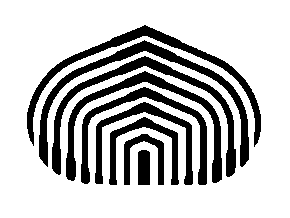
\includegraphics[scale=0.5,type=png,ext=.png,read=.png]{imagenes/cebolla} \\

% Encabezado
\textsc {\large UNIVERSIDAD SIMÓN BOLÍVAR} \\
\textsc{\bfseries DECANATO DE ESTUDIOS PROFESIONALES\\
COORDINACI'ON DE INGENIER'IA DE LA COMPUTACI'ON}

\bigskip
\bigskip
\bigskip
\bigskip
\bigskip
\bigskip
\bigskip
\bigskip
\bigskip

% Title/Titulo
% Aqui ponga el nombre de su proyecto de grado/pasantia larga
\textsc{\bfseries Desarrollo de un prototipo de robot humanoide que busque, encuentre y patee una pelota de forma autónoma e inteligente}

\bigskip
\bigskip
\bigskip
\bigskip
\bigskip

% Author and supervisor/Autor y tutor
\begin{minipage}{\textwidth}
\centering
Por: \\
Jennifer Dos Reis De Nóbrega \\ Juliana Le\'on Quinteiro\\

\bigskip
\bigskip
\bigskip

Realizado con la asesoría de: \\
Ivette Carolina Mart\'inez 
\end{minipage}

\bigskip
\bigskip
\bigskip
\bigskip
\bigskip
\bigskip
\bigskip
\bigskip
\bigskip

% Bottom half
{PROYECTO DE GRADO \\ Presentado ante la Ilustre Universidad Simón Bolívar \\
como requisito parcial para optar al título de \\ Ingeniero en Computación} \\

\bigskip
\bigskip
\vfill

% Date/Fecha 
{\large \bfseries Sartenejas, 
%FECHA
Noviembre 2014}

\end{center}
\end{titlepage}


% Pagina de acta final (vacio)
%\pagestyle{empty}
%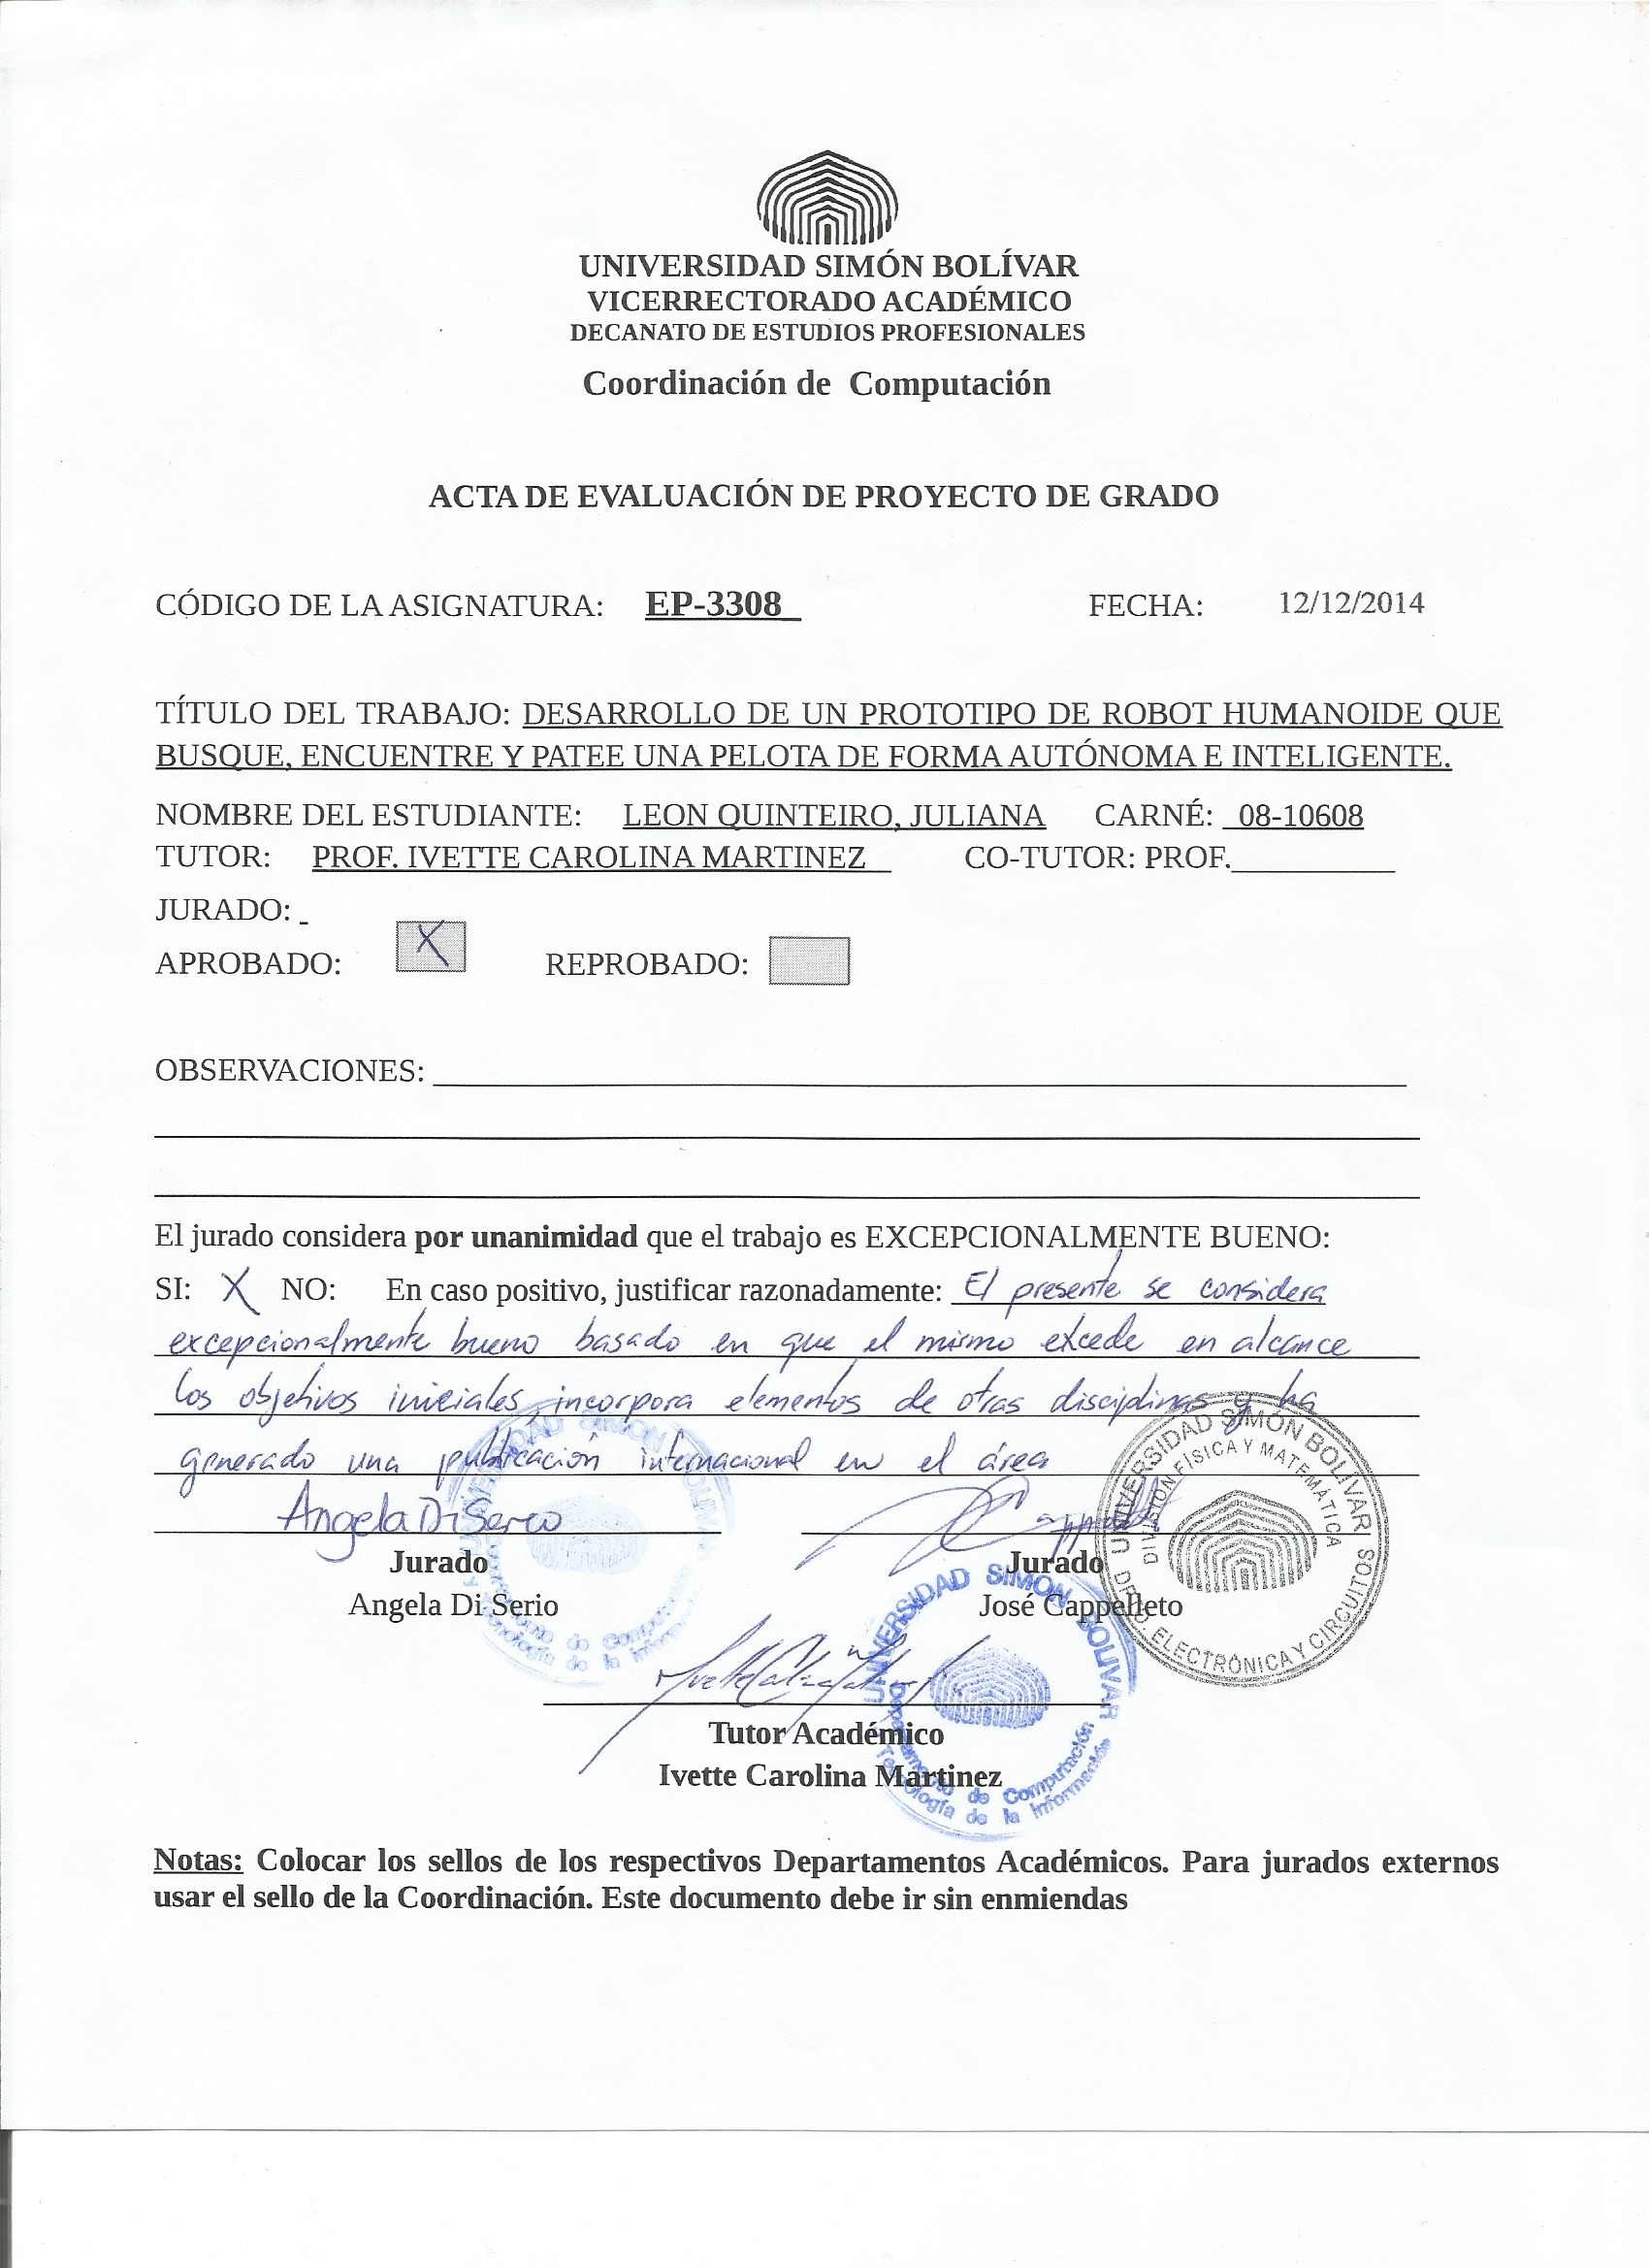
\includegraphics[width=\textwidth, height=\textheight]{figures/acta.jpg}

\setcounter{secnumdepth}{3}
\setcounter{tocdepth}{4}

% Define encabezado numeros romanos y como se separan los captiulos y las
% secciones
\addtolength{\headheight}{3pt}
\pagenumbering{roman}
\pagestyle{fancyplain}

\renewcommand{\chaptermark}[1]{\markboth{\chaptername\ \thechapter:\,\ #1}{}}
\renewcommand{\sectionmark}[1]{\markright{\thesection\,\ #1}}

\onehalfspacing

\lhead{}
\chead{}
\rhead{}
\renewcommand{\headrulewidth}{0.0pt}
\lfoot{}
\cfoot{\fancyplain{}{\thepage}}
\rfoot{}


% Pagina de resumen
\setcounter{page}{4}
\begin{center}
	{\bf Resumen} \pdfbookmark[0]{Resumen}{resumen} % Sets a PDF bookmark for the dedication
\end{center}	

%RoboCup \cite{robotcup} es una competencia de fútbol, iniciada en 1997, donde contribuyen las áreas de robótica, investigación e inteligencia artificial. Entre sus categorías se encuentra RoboCup Soccer \cite{robotcupsoccer}, la cual consiste en la participación de pequeños robots humanoides que se enfrentan a otro equipo para jugar fútbol.

En este proyecto se describe la construción de Junny, un robot humanoide autónomo e inteligente de $38 cm $ de alto, capaz de detectar la ubicación de una pelota y acercarse a ella para patearla con dirección al arco. Los objetivos de Junny están inspiradas en la liga RoboCup Soccer de la competencia RoboCup.

Junny ha sido ensamblado con las piezas del kit Bioloid Premium del fabricante Robotis. Del kit se ha excluido la tarjeta CM-510 para sustituirla por la tarjeta controladora Arbotix, la cual controla los 16 motores que permiten el movimiento de las extremidades del robot. Se ha incluido un mini computador Raspberry Pi, con su cámara, %\cite{raspberrycam},
de esta forma el robot ha adquirido la posibilidad detectar la posición de la pelota y el arco de forma autónoma. Se añadieron dos micro servomotores analógicos para ejecutar el movimiento de la c\'amara, estos son controlados por la tarjeta Arbotix. 

En la Raspberry Pi se ejecuta un solo programa encargado de detectar la posición de la pelota y decidir qué movimientos son necesarios para llegar a ella. La manera de elegir las acciones se ha realizado con aprendizaje por reforzamiento. Para filtrar y procesar la imagen se ha usado la segmentaci\'on por regiones para la detecci\'on de la pelota, con ayuda de las librerías OpenCv. % \cite{opencv}. 

La Arbotix, además de controlar los motores para ejecutar los movimientos deseados, se encarga de monitorizar la velocidad angular del robot, para ello usa el sensor Gyro de Robotics. Con esta información Junny puede deducir si se ha caído y levantarse. 
% Si detecta un desbalance de un cierto porcentaje 

Todos estos componentes deben ser coordinados para que se logre cumplir la tarea de seguir y patear la pelota. Por ello se hizo necesaria la comunicación entre la Arbotix y la Raspberry Pi. La herramienta 
empleada para ello ha sido el \gls{framework} \gls{ROS} (Ros Operating System). %\cite{ros}. 

Finalmente se obtuvieron los siguientes resultados, un robot aut\'onomo e inteligente que es capaz de reconocer la pelota, desplazarse hasta ella y patearla con direcci\'on al arco. Con la aplicaci\'on de aprendizaje por reforzamiento, se obtuvo un 100\% de aciertos, con una tasa de eficiencia de $0.72$ que es el n\'umero de acciones optimas entre las acciones realizadas. De los experimentos completos con la orientaci\'on al arco se obtuvo un 53 \% de orientaciones correctas con resultado de gol.

\textbf{Palabras claves}: Rob\'otica, Aprendizaje por reforzamiento, Humanoide, ROS, Arbotix.




% Pagina de dedicatoria (opcional)
%\pagebreak

\setcounter{page}{5}

\vspace*{8cm} 
\pdfbookmark[0]{Dedicatoria}{dedicatoria} % Sets a PDF bookmark for the dedication
\begin{center} 
\large DEDICATORIA
\end{center}
\newpage


% Pagina de agradecimientos (opcional)
\setcounter{page}{6}

\chapter*{Agradecimientos
\markboth{Agradecimientos}{Agradecimientos}}
\pdfbookmark[0]{Agradecimientos}{agradecimientos}

\bigskip

AGRADECIMIENTOS



% Crea la tabla de contenidos
\tableofcontents

% Crea la lista de cuadros
\listoftables

% Crea la lista de figuras
\listoffigures

% Crea la lista de codigos fuentes
%\lstlistoflistings

\clearpage

% Define encabezado en numeros arabicos  
\pagenumbering{arabic}

\fancyhf{} % Redefine el encabezado 
\lhead{}
\chead{}
\rhead{\fancyplain{}{\thepage}}
\renewcommand{\headrulewidth}{0.0pt}
\lfoot{}
\cfoot{}
\rfoot{}

\doublespacing

% Incluye los archivos deseados - El contenido de su proyecto de grado/pasantia larga.
\chapter{Introducción}\label{intro}

\pdfbookmark[0]{Introducción}{introduccion} % Sets a PDF bookmark for the dedication

\label{sect:justificacion}
RobotCup \cite{robotcup} es una competencia de fútbol iniciada desde 1997 donde contribuyen las áreas de robótica, investigación e inteligencia artificial. Entre sus categorías se encuentra RobotCup Soccer \cite{robotcupsoccer}, la cual consiste en la participación de pequeños robots humanoides que se enfrentan a otro equipo para jugar fútbol. El objetivo de esta competencia es lograr que en el año 2050 el equipo campeón logre vencer al ganador del año en la copa mundial de la FIFA (International Federation of Association Football). Las destrezas de robots con forma de humanos (como son caminar, percibir el mundo y tomar alguna acción sobre él) suelen ser más complejas de lo que se puede pensar. Una de las más avanzadas muestras en el área es el robot ASIMO \cite{asimo}, creado por la compañía Honda, cuyos últimos avances incluyen la predicción de trayectoria de objetos para poder esquivarlos.

En este proyecto se presenta un robot humanoide (Debupa) de tamaño pequeño (38 cm de altura) cuyos objetivos estan basados en las reglas de la competencia RobotCup. En artículos de este mismo enfoque se puede encontrar el trabajo de Sven Behnke cuyo título es “See, walk, and kick: Humanoid robots start to play soccer” donde se describe la construcción del equipo de robots que participaron en la RobotCupSoccer en el a\~no 2006. El artículo cubre el diseño mecánico y electrónico, además el software utilizado para la percepción, control de comportamiento, comunicación y simulación de los robots. \cite{paper}.

Existen equipos que han participado durante varios años consecutivos en la competencia Robocup, logrando mejoras en sus diseños y técnicas; tal es el caso del equipo MRL que ha participado en los años 2011, 2012, 2013 y 2014 en la categoría “Humanoid League”, han iniciado con el hardware del robot DARwIn-OP y con el tiempo han modificado los componentes electrónicos para agregar eficiencia y estabilidad. Para el balance han utilizado un giróscopio y sensores de aceleración, y para la visión una cámara conectada por usb al CPU principal \cite{paper1}.

En el desarrollo de habilidades más específicas con respecto a la competencia RobotCup Soccer, en el artículo de investigación de Seung-Joon Yi, Stephen McGill y Daniel D. Lee  \cite{paper2}, se refieren a dos posibles estrategias para el pateo de la pelota donde los factores fundamentales para un buen desempeño es la fuerza y la rapidez con que se patea, los investigadores ponen en pr\'actica dos estrategias de pateo en distintas circunstancias del juego basado en la cinemática y dinámica de equilibrar el cuerpo al momento de realizar el pateo.

El objetivo general de este proyecto se basa en construir un prototipo de robot humanoide que sea capaz de detectar la cercanía
de una pelota, acercarse a ella y patearla, reincorporandose a la posicion de pie en caso de perder el equilibrio y caer
mientras camina. Para cumplir con este objetivo se ha desglosado un conjunto de objetivos específicos que se describen 
a continuación: 

\begin{enumerate}
\item  Diseño y construcción de un humanoide con piezas del kit de robótica Bioloid Premium, sustituyendo su tarjeta controladora
CM-530 por la tarjeta de software libre ArbotiX para controlar los motores Dynamixel y otros sensores.
\begin{enumerate}
\item Instalación y configuración de la tarjeta ArbotiX.
\item Instalación y configuración de la tarjeta Raspberry Pi.
\item Instalación y configuración de la cámara Raspberry Pi.
\item Instalación de servomotores  para el movimiento de la cámara
\item Instalación del giroscopio Gyro.
 
\end{enumerate}
\end{enumerate}

\begin{enumerate}
\item Detección de la pelota
\begin{enumerate}
\item  Captura de imagen con la cámara Raspberry Pi a través de la librería raspicam cv.
\item Procesamiento de la imagen para extraer información de la posición de la pelota con las librerías de OpenCV.
\end{enumerate}

\end{enumerate}

\begin{enumerate}
\item Búsqueda de la pelota y pateo de la misma. 
\begin{enumerate}
\item Creación de las poses necesarias para caminar, girar, levantarse y patear usando el software pypose.
\item Programación de transiciones de movimientos.
\item Control de servomotores para el movimiento de la cámara.
\item Establecer mecanismo de comunicación entre la tarjetas ArbotiX y Raspberry Pi.  
\item Programación de algoritmo de planificación de acciones que lleve al humanoide a acercarse a la pelota.
\item Detección de movimientos angulares bruscos que sugieran una caída, a través de la lectura del giroscopio
\item Identificación del momento en que la pelota se encuentre en una zona adecuada para patear.
\end{enumerate}
\end{enumerate}

En el capítulo (\ref{chapter:Tecnologias_utilizadas}) se describen los componentes de hardware usados para construir el humanoide; luego en la sección \ref{sec:Estru}
se explica cómo se unieron esas piezas. Con respecto a la parte de programación, en la secci\'on \ref{sec:Movimientos} se describe c\'omo se logró constituir los movimientos necesarios para que el humanoide cumpla sus objetivos, mientras que en la secci\'on \ref{sec:resultados} se muestran los resultados experimentales. Las herramientas y técnicas  que  permitieron lograr  la detección de la pelota se detallan en la secci\'on \ref{sec:vision_del_robot}. También se describe la discretización del ambiente para reducir el n\'umero de estados. La comunicación de las tarjetas Arbotix y Raspberry Pi para que puedan trabajar en conjunto se explica en la secci\'on \ref{sec:integracion_de_componentes}  y consideraciones especiales en la secci\'on \ref{sec:consideraciones}.


% Marco Teorico.
\chapter{Marco teórico} \label{chap:marco_teorico}
\vspace{5 mm}
En este capítulo se presentan los conceptos que conforman la base teórica para comprender este trabajo. Primero se brinda una descripción de los términos relativos a la robótica y las partes principales de un robot. Posteriormente se describen algunos conceptos que tienen que ver con la robótica inteligente, como los paradigmas, la inteligencia y la visión artificial para la detección de objetos. 
\section{Robótica} \label{sect:robotica}
 
Para definir un lenguaje formal se requiere describir:
\begin{itemize}
\item{\textbf{Robot:} Es un agente artificial, activo, cuyo entorno no es el mundo físico. El término activo descarta de esta definición a las piedras, el término artificial descarta a los animales, y el término físico descarta a los agentes de software puros o softbots, cuyo entorno lo constituyen los sistemas de archivos, bases de datos y redes de cómputo. \cite{peterNorvig}}

\item{\textbf{Robótica:} Es la rama de la tecnología que se encarga del diseño, construcción, operación y aplicación de los robots. \cite{oxfordRobotics}}

\item{\textbf{Sensores:}  Son los encargados de percibir el ambiente que rodea al robot. Según Murphy R.R son dispositivos que miden algún atributo del mundo. Un sensor recibe energía del entorno (sonido, luz, presión, temperatura, etc) y transmite una señal a una pantalla o computador ya sea de forma análoga o digital. \cite{AiRobotics}}

\item{\textbf{Actuador:}  Es aquella parte del robot que convierte comandos de software en movimientos físicos.  \cite{peterNorvig}}

\item{\textbf{Servomotor:}  Es un motor eléctrico, considerado como actuador, que permite ser controlado tanto en velocidad como en posición. }

\item{\textbf{Giróscopio:} Es un sensor utilizado para medir y mantener la orientación, se mide a través del momento angular. \cite{gyro1}}
\end{itemize}

%****************************************************************************************/
\section{Robótica Inteligente (Agentes Inteligentes)} \label{sect:AgentesInteligentes}
\subsection{Paradigmas de robótica}
En la robótica inteligente, según Robin Murphy, existen tres paradigmas en los cuales se clasifica el diseño de un robot inteligente, estos paradigmas pueden ser descritos de dos maneras: la relación entre las primitivas básicas de la robótica, percibir, planificar, actuar o de la forma en que los datos son percibidos y distribuidos en el sistema.

Percibir se refiere al procesamiento útil de la información de los sensores del robot. Planificar, cuando con información útil, se crea un conocimiento del mundo y se generan ciertas tareas que el robot podría realizar. Por último actuar consiste en realizar la acción correspondiente con los actuadores del robot para modificar el entorno. 

\subsubsection{ Paradigma Jerárquico}

Este paradigma es secuencial y ordenado. Primero el robot percibe el mundo y construye un mapa global. En base al mapa ya percibido y con “los ojos cerrados”, el robot planifica todas tareas necesarias para lograr la meta. Luego ejecuta la secuencia de actividades según la planificación realizada. Una vez culminada la secuencia se repite el ciclo percibiendo el mundo, planificando y actuando. \cite{AiRobotics}

\subsubsection{Paradigma Reactivo}
El paradigma reactivo omite por completo el componente de la planificación y solo se basa en percibir y actuar. El robot puede mantener un conjunto de pares percibir-actuar, estos son llamados comportamientos y se ejecutan como procesos concurrentes. Un comportamiento toma datos de la percepción del mundo y los procesa para tomar la mejor acción independientemente de los otros procesos. \cite{AiRobotics}

\section{Inteligencia Artificial} \label{sect:Inteligencia_Artificial}
La inteligencia artificial es un término relacionado con la computación y la robótica que ha tenido varias definiciones, ocho de ellas, las cuales nacieron a finales del siglo XX, se encuentran organizadas en \cite{peterNorvig} bajo cuatro categorías: pensar y actuar de forma humana, pensar y actuar de forma racional. Con ello se puede entender que la inteligencia artificial tiene que ver con lograr que un robot resuelve problemas de manera inteligente, es decir, de manera que parezca que el razonamiento y comportamiento humano las ha resuelto.  

\subsection{ Aprendizaje de Máquinas}
El aprendizaje de máquinas es un área de la inteligencia artificial que está relacionada con la pregunta de cómo construir programas de computadora que automáticamente mejoren con la experiencia. Se dice que un programa aprende de la experiencia E con respecto a una tarea T y desempeño P si el desempeño en la tarea T, medido por P, mejora con con la experiencia E \cite{Mitchell}.
\subsection{Aprendizaje por reforzamiento}
El aprendizaje por reforzamiento es un tipo de aprendizaje de máquinas que se basa en un sistema de recompensas y penalizaciones. Las recompensas se pueden dar en cada estado o una sola vez al llegar al estado final.

El objetivo del agente es aprender de las recompensas para escoger la secuencia de acciones que produzca la mayor recompensa acumulada. \cite{Mitchell}

El agente existe en un entorno descrito por algunos estados S. Puede ejecutar un conjunto de acciones A. Cada vez que ejecuta una acción $a_t$ en algún estado $s_t$ el agente recibe una recompensa $r_t$. El objetivo es aprender una política $\pi$ : S $\to$ A que maximice la suma esperada de esas recompensas con descuento exponencial de las recompensas futuras. \cite{Mitchell} El resultado de tomar las acciones puede ser determinista o no, en el caso de este proyecto no es determinista, es decir, existen porcentajes de probabilidad de pasar a un estado u otro al tomar una acción en un estado en particular.  
\subsection{ Q- learning}

Es un método de aprendizaje por reforzamiento que, dado un estado, compara las utilidades esperadas de las posibles acciones a tomar sin necesidad de saber el estado resultante, por tanto no se necesita tener un modelo del entorno \cite{peterNorvig}.

La forma de aprender la política $\pi$ : S $\to$ A es de forma indirecta, a través de la función $Q(s,a)$. La función esta definida como el valor de la máxima recompensa acumulada con descuento que puede ser alcanzada desde el estado $s$ y aplicando $a$ como la primera acción. Es decir, el valor de Q es la recompensa recibida inmediatamente 


\section{Visión Artificial} \label{sect:Vision_Artificial}

Una manera de obtener información del ambiente es con la visión artificial. Esta consiste en usar un dispositivo (cámara) que
capta el espectro electromagnético y produce una imagen. La representación de la imagen se almacena como una matriz de píxeles,
cada píxel es un elemento que guarda información de una región en el espacio captado. Si se usa una cámara de luz, la información
de cada píxel será el color. \cite{AiRobotics}  

Por lo general luego de obtener una imagen se requiere extraer información de ella, por lo cual se han desarrollado diferentes algoritmos y t\'ecnicas que ayudan en esta tarea. En la sección \ref{sec:Segmentacion} se describe la t\'ecnica de segmentaci\'on por regiones, que es la utilizada en esta proyecto. 

Por otro lado, existen varios algoritmos que se dedican a la transformación de las imágenes para reducir
ruidos, compensar problemas de iluminación, extraer formas, identificar objetos, entre otros. En esta sección se describen dos de las técnicas de transformación para reducir el ruido basadas en la dilatación y erosión de la imagen (secci\'on \ref{sec:Transfor}). 
 
\subsection{Segmentaci\'on por regiones}\label{sec:Segmentacion}

La pr\'actica m\'as general en visi\'on de computadoras aplicado a rob\'otica es la identificaci\'on de regiones por un color particular, este proceso se llama segmentaci\'on por regiones. El algoritmo b\'asico consiste en identificar todos los p\'ixeles en una imagen que forman parte de una regi\'on y luego navegar al centro de la regi\'on. El primer paso es identificar todos los p\'ixeles en la imagen que compartan un rango de valores con el color particular y agruparlos, aquellos p\'ixeles que no compartan el color son descartados \cite{BookOpenCv}. 

\subsection{Filtros}
El filtrado de imágenes es una técnica para la transformación de imágenes, que consiste en destacar  sus características más relevantes en base a un propósito en particular. 

Generalmente en la tarea de extracción de información de una imagen se utilizan filtros para descartar zonas o características que no son importantes para el patrón deseado y para determinar el área deseada ya sea por patrones de forma o color.

En la investigación, los algoritmos de filtrado aplicados a las imágenes fueron: Clausura Morfológica y Apertura Morfológica, filtros que aplican las técnicas de erosión y dilatación a las imágenes.

\subsection{Transformaciones Morfológicas}\label{sec:Transfor}
Las transformaciones morfológicas básicas son llamadas dilatación y erosión, se utilizan en 
amplia variedad de contextos como la eliminación del ruido, aislamiento de elementos individuales y elementos de unión dispares
en una imagen.\cite{BookOpenCv}

\subsubsection{Dilatación}
La dilatación es una convulsión (algo que se le aplica a toda la imagen) entre alguna imagen (o región de una imagen), que llamaremos A y un núcleo que llamaremos B, el núcleo, que puede ser de cualquier forma o tamaño, tiene un solo punto de anclaje definido. Para mayor claridad el n\'ucleo es esencialmente una matriz de tamaño fijo  de coeficientes numéricos junto con un punto de anclaje en dicha matriz, que normalmente se encuentra en el centro . Muy  a menudo, el núcleo es un pequeño cuadrado o disco sólido. El núcleo puede ser pensado como una plantilla  o m\'ascara, y su efecto para la dilatación tal como un operador de máximo local sobre la imagen, se calcula el m\'aximo valor de los píxeles común a B y reemplazamos el píxel de la imagen en el punto de anclaje con ese valor máximo. Esto causa regiones brillantes dentro de una imagen y la hacen crecer. Este crecimiento es el origen del término `` operador de dilatación" \cite{BookOpenCv}. 

\begin{figure}[hbtp]

\centering
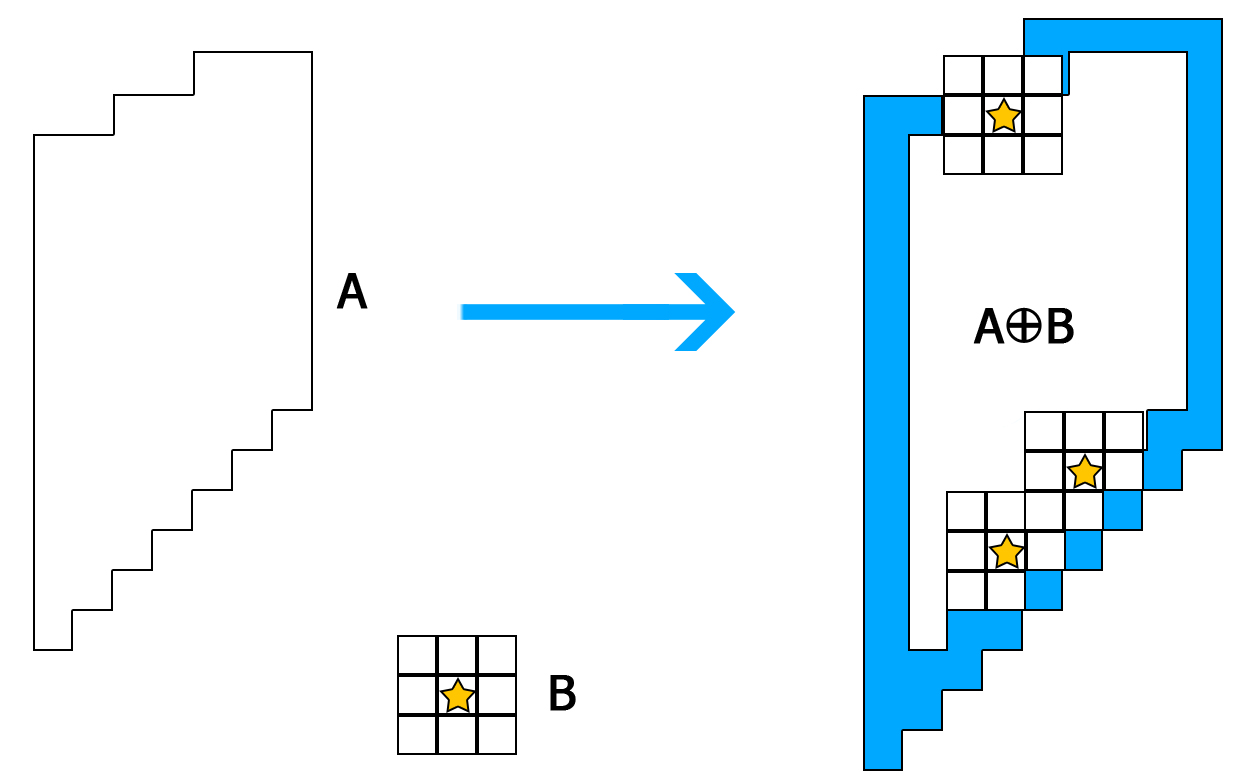
\includegraphics[scale=0.2]{imagenes/erosion-model.jpg}
\caption{Dilatación}
\end{figure}

\subsubsection{Erosión}
La erosión es la operación inversa a la dilatación. Esta acción del operador es equivalente a el cálculo de un mínimo local sobre el área del núcleo. La erosión genera una nueva imagen a partir de la original, utilizando el siguiente algoritmo: como el núcleo B es analizado sobre la imagen, se calcula el mínimo valor del píxel superpuesto por B y se reemplaza el píxel de la imagen con un punto de anclaje de valor mínimo \cite{BookOpenCv}. 
V\'ease en la figura \ref{fig:erosion}

\begin{figure}[hbtp]
\centering
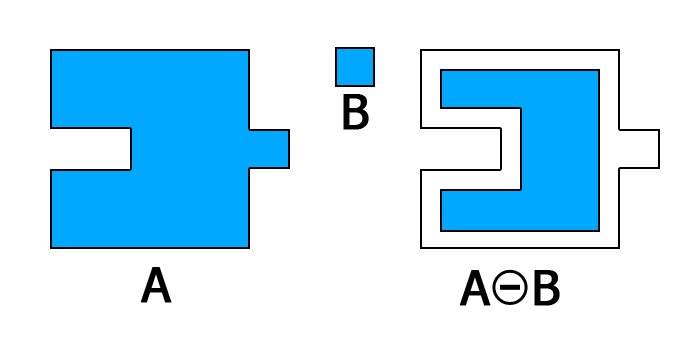
\includegraphics[scale=0.5]{imagenes/erosion.jpg}
\caption{Erosión}
\label{fig:erosion}
\end{figure}





\chapter{Construcion de un robot humanoide}\label{chapter:introAdesarrollo}

INTRO A TODO EL DESARROLLO




% Seccion de Diseno y construccion 

%%\chapter{Integración de componentes}
\label{chapter:diseno}
\section{Diseño y Construcción}

El primer paso ha sido la construcci\'on de la parte física del robot. Para tal fin se procedió a la elección del diseño y ensamblaje de las piezas. En la sección \ref{subsection:componentes} se describe cada uno de los componentes utilizados para armar el robot, y luego, en la secci\'on \ref{subsection:construccion} se explica cómo se integraron esas piezas para obtener un humanoide adaptado a los objetivos de este proyecto.

\label{subsection:componentes}
\subsection{Componentes de hardware}
A continuación se presenta una descripción de todos los elementos utilizados para la construcción del robot humanoide. 

\begin{itemize}
\item Bioloid Premium kit: Es un kit de robótica con piezas modulares que permite armar diferentes tipos de robot pero principalmente humanoides. Su empaque se puede observar en la figura ~\ref{fig:kit}. El fabricante, ROBOTIS, incluye un manual con varios modelos de robots con instrucciones de ensamblaje. Provee una tarjeta controladora, CM-510, a la que se conectan los motores Dynamixel y algunos sensores que se programan a través de la interfaz de ‘RoboPlus’\cite{robotics}. 

\end{itemize}

\begin{figure}[hbtp]

\centering
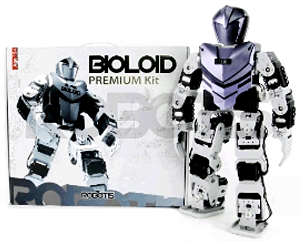
\includegraphics[scale=0.5]{imagenes/product_bioloid17.png}
\caption{Bioloid Premium Kit}
\label{fig:kit}
\end{figure}

\begin{itemize}

\item Motores Dynamixel Ax-12+: Son actuadores inteligentes y modulares que incorporan un reductor de engranajes, un motor DC de presión y un circuito de control con funcionalidad de red lo cual permite formar series de motores (figura ~\ref{fig:motoresDc}), todo en un solo paquete \cite{manual}. 
\end{itemize}

\begin{figure}[hbtp]

\centering
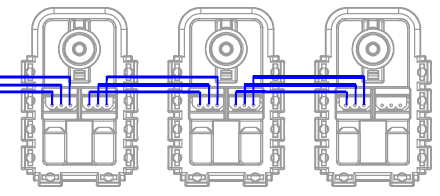
\includegraphics[scale=0.5]{imagenes/AX-12_serie.png}
\caption{Motores Dynamixel conectados en serie}
\label{fig:motoresDc}
\end{figure}

\begin{itemize}
\item Gyro: Es un giroscopio de la marca Robotis que mide la velocidad angular. Se encuentra diseñado para mantener el balance del robot y ser usado para otras aplicaciones de movimiento\cite{gyro}. En figura ~\ref{fig:gyro} se puede observar su estructura.  

\end{itemize}

\begin{figure}[hbtp]
\centering
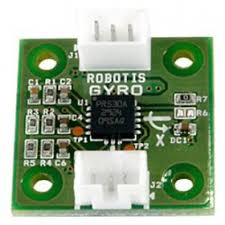
\includegraphics[scale=0.35]{imagenes/gyro.jpg}
\caption{Sensor Gyro}
\label{fig:gyro}
\end{figure}

\begin{itemize}
\item Arbotix: El controlador ArbotiX es una solución de control avanzado para manejar algunos tipos de servos Dynamixel y robots
basados en Bioloid. Incorpora un potente microcontrolador AVR, radio inalámbrica XBEE, conductores de motor dual, y cabeceras
de estilo servo de 3 pines para entrada/salida digital y analógica \cite{arbotix}.

\end{itemize}

%\begin{figure}[hbtp]
%\centering
%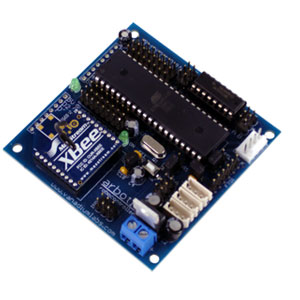
\includegraphics[scale=0.5]{imagenes/ARBOTIX.JPG}
%\caption{Tarjeta controladora ArbotiX}
%\end{figure}

\begin{itemize}
\item FTDI (Future Technology Devices International) : Es una tarjeta controladora  (figura ~\ref{fig:ftdi}) que ofrece el servicio de conversión de  datos de USB a UART. Permite la comunicación entre diferentes dispositivos \cite{ftdi}.

\end{itemize}

\begin{figure}[hbtp]
\centering
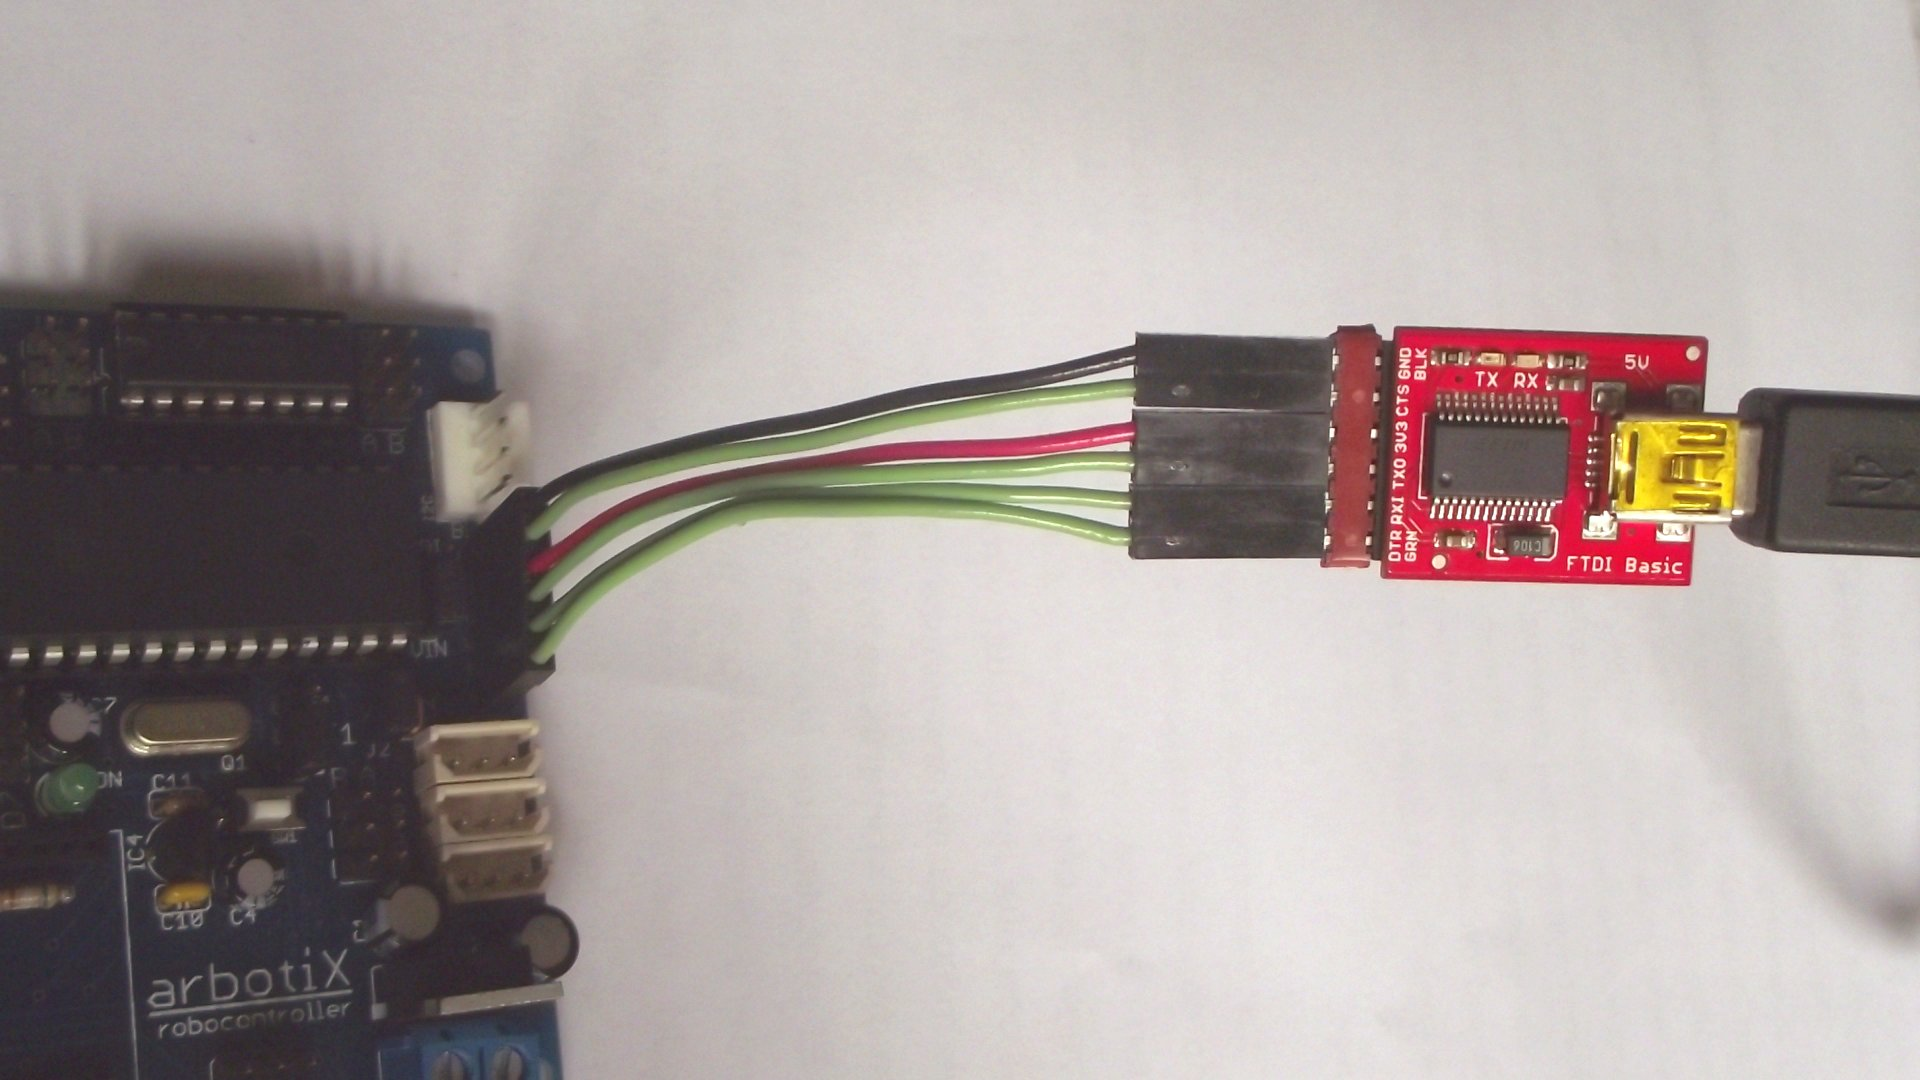
\includegraphics[scale=0.06]{imagenes/DSCF1162.jpg}
\caption{Chip FTDI conectado a la tarjeta Arbotix}
\label{fig:ftdi}
\end{figure}

\begin{itemize}
\item Extensor de puertos bioloid : Permite aumentar el número de cadenas de servos conectados a la tarjeta. (figura ~\ref{fig:ext}) \cite{hub} 
\end{itemize}

\begin{figure}[hbtp]
\centering
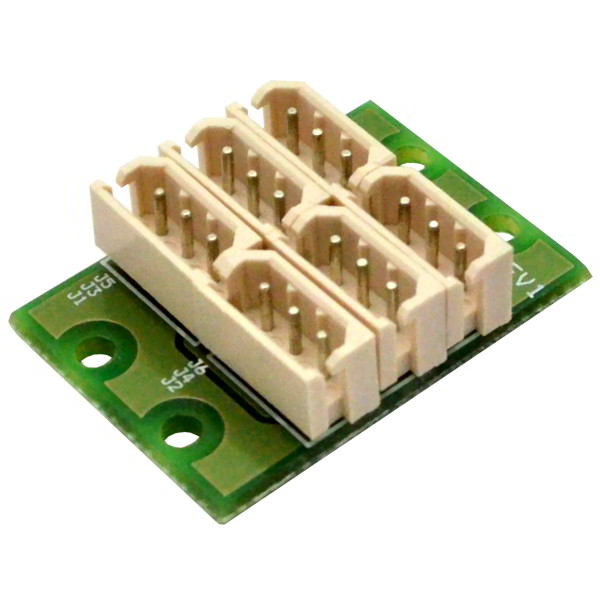
\includegraphics[scale=0.15]{imagenes/Dynamixel-AX-MX-6-Port-Extension-Hub-600x600.jpg}
\caption{Extensor de puertos bioloid}
\label{fig:ext}
\end{figure}

\begin{itemize}
\item Servo motor anal\'ogico micro TG9 e: Es un pequeño servomotor  (figura ~\ref{fig:Servo}) cuyo torque alcanza 1.50 kg-cm y una velocidad de 60 por segundo. Permite ser controlado en posición en un rango de 180. \cite{microservo}  

\end{itemize}

\begin{figure}[hbtp]
\centering
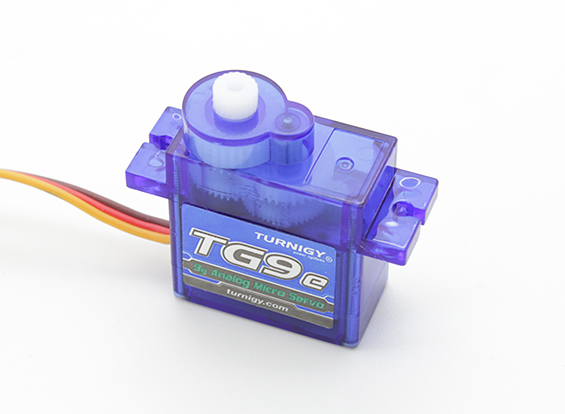
\includegraphics[scale=0.2]{imagenes/turnigy.jpg}

\caption{Servo motor analógico}

\label{fig:Servo}
\end{figure}

\begin{itemize}
\item Raspberry Pi: La Raspberry Pi (figura ~\ref{fig:Raspe}) es un ordenador del tamaño de una tarjeta de crédito a la que se puede conectar un televisor y un teclado. Se trata de un pequeño ordenador capaz de ser utilizado en proyectos de electrónica y para muchas de las tareas que una PC de escritorio hace, como hojas de cálculo, procesadores de texto y juegos \cite{raspberry}. 

\end{itemize}

%imagen tomada de: %http://rayhightower.com/blog/2012/12/03/ruby-on-raspberry-pi/
\begin{figure}[hbtp]
\centering

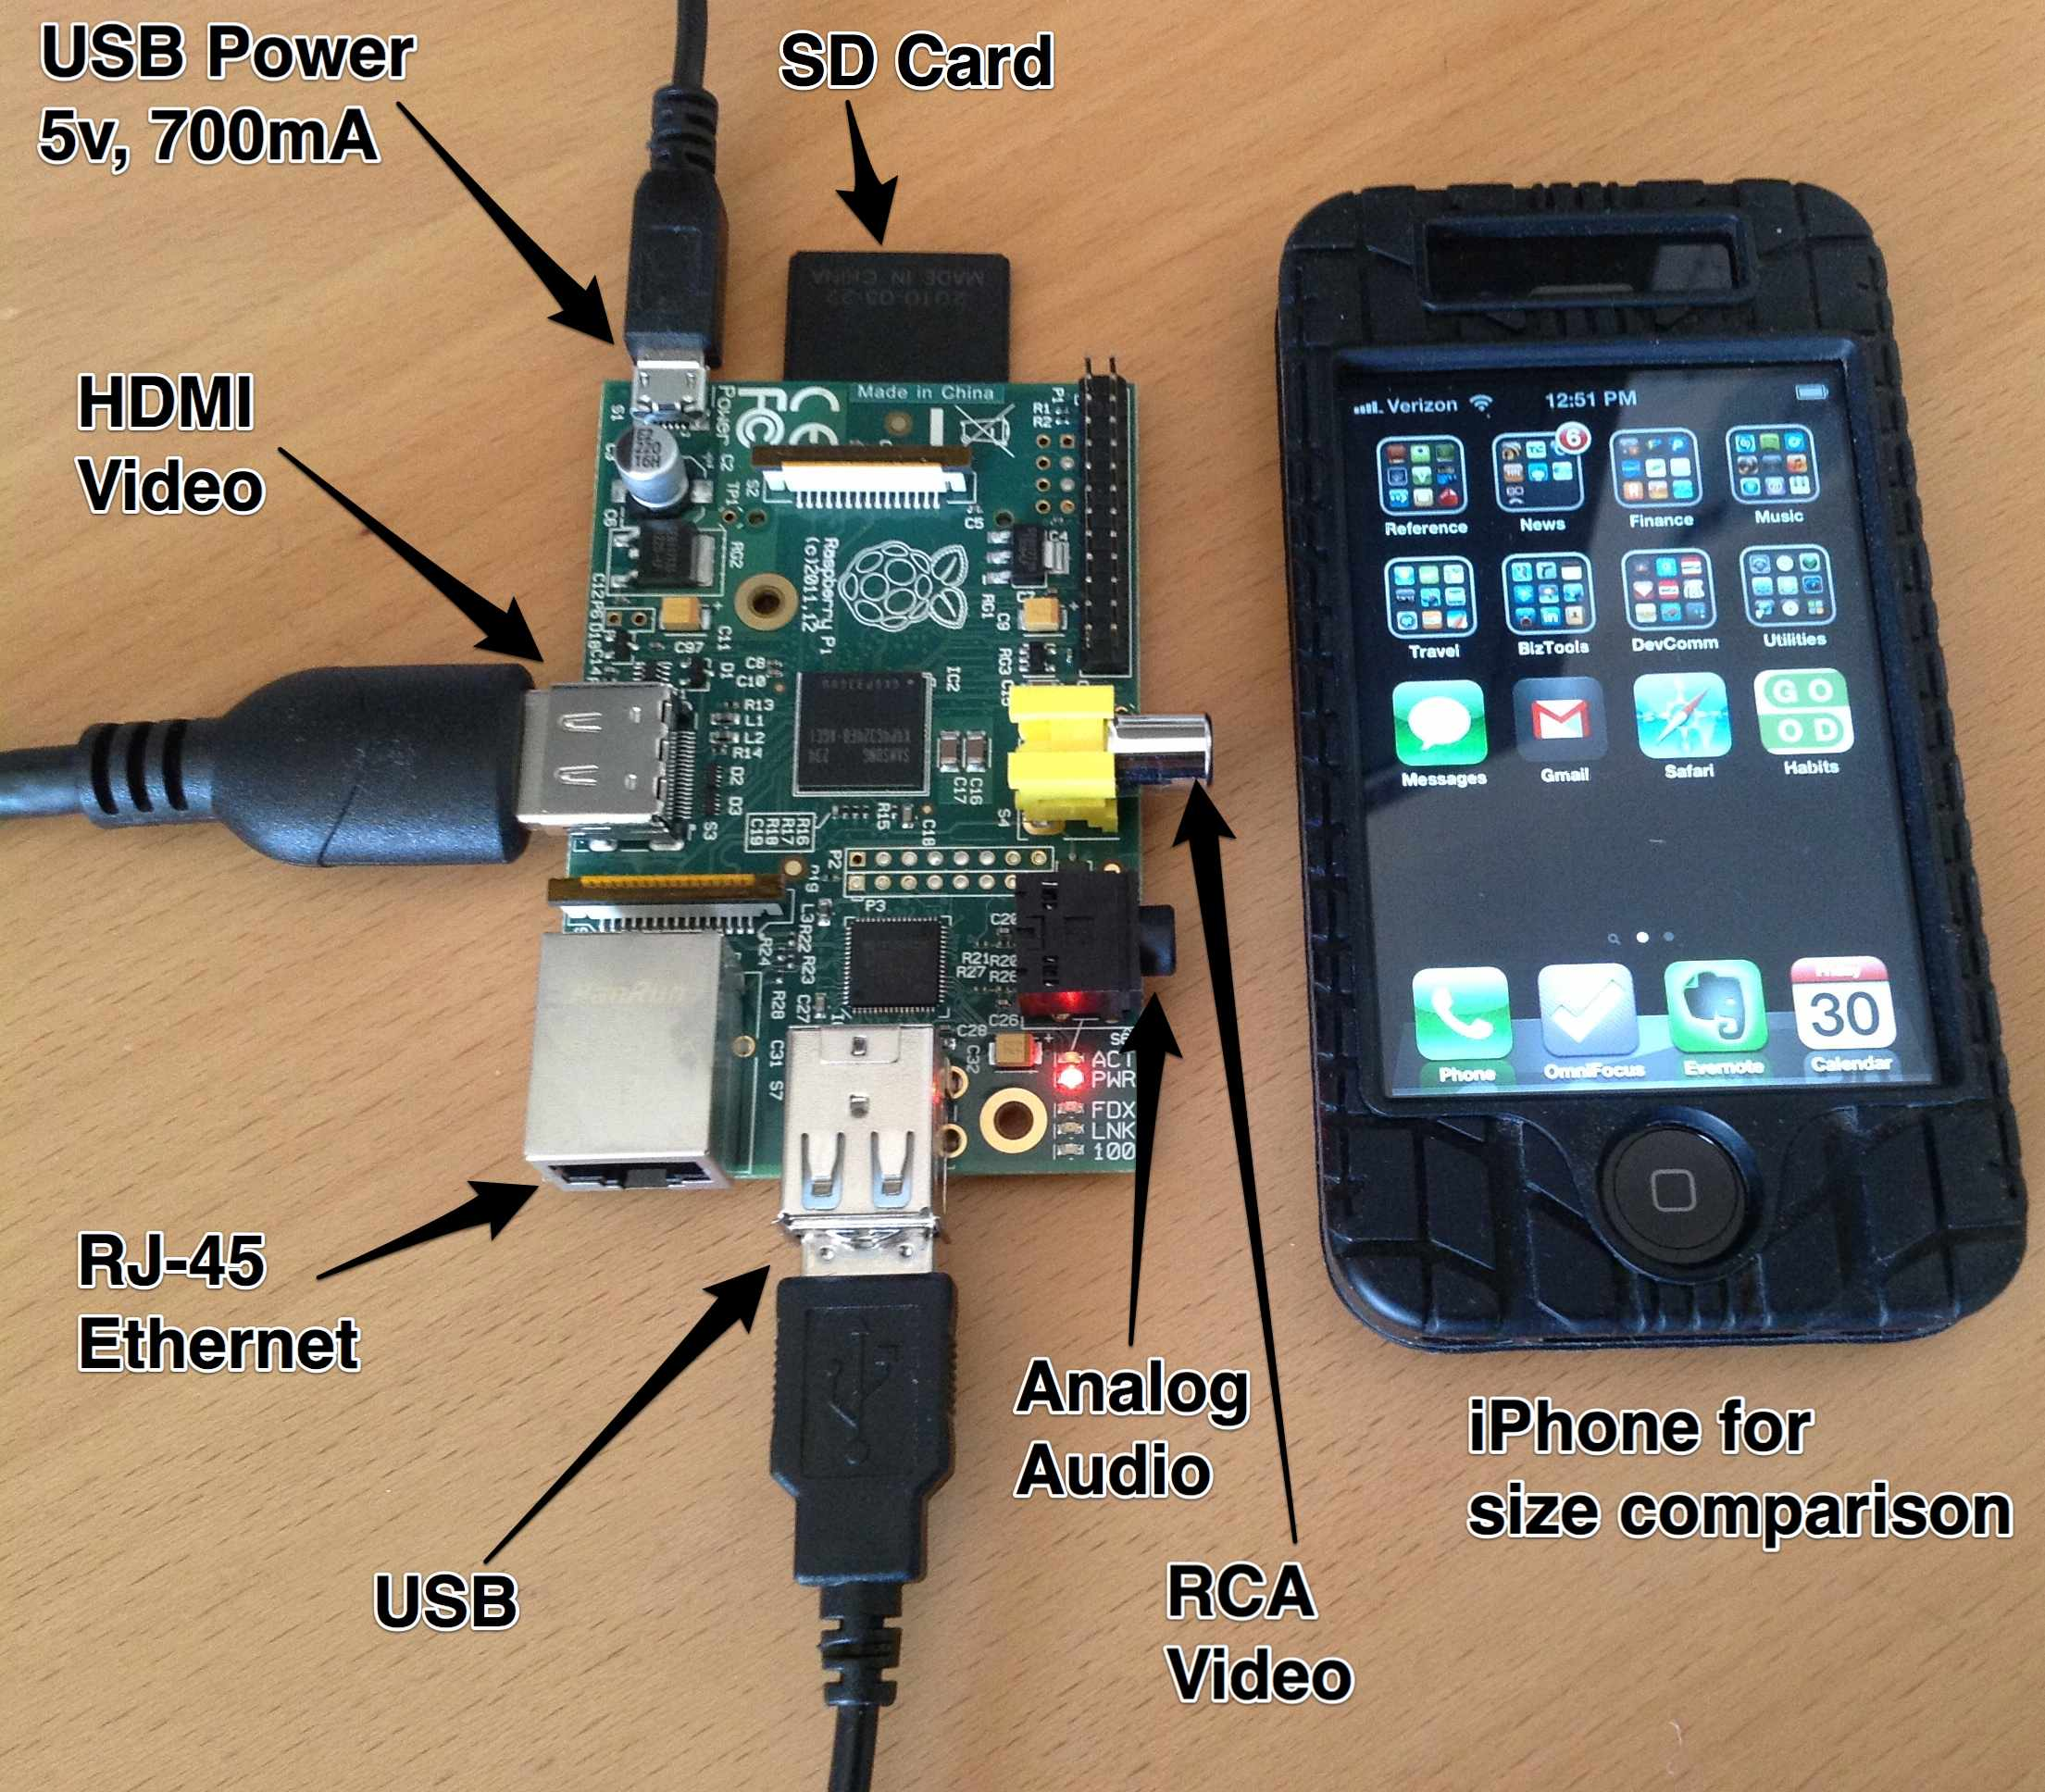
\includegraphics[scale=0.1]{imagenes/raspberry_pi_iphone.jpg}
\caption{Tarjeta Raspberry Pi con descripción de los puertos}
\label{fig:Raspe}
\end{figure}

\begin{itemize}
\item C\'amara Raspberry Pi: Es un sensor encargado de captar imagenes y grabar videos de alta definicion. Se conecta a la Raspberry Pi con un cable de cinta plana de 15 cm en el puerto CSI. Tiene 5 megapíxeles de foco fijo que soporta los modos de vídeo de 1080x30, 720x60 y VGA90. Puede ser manejada con las librerías MMAL, V4L u otras librerías de terceros como la de Python.(figura ~\ref{fig:came}) \cite{raspberrycam} %(http://www.raspberrypi.org/products/camera-module/)

\end{itemize}

\begin{figure}[hbtp]
\centering
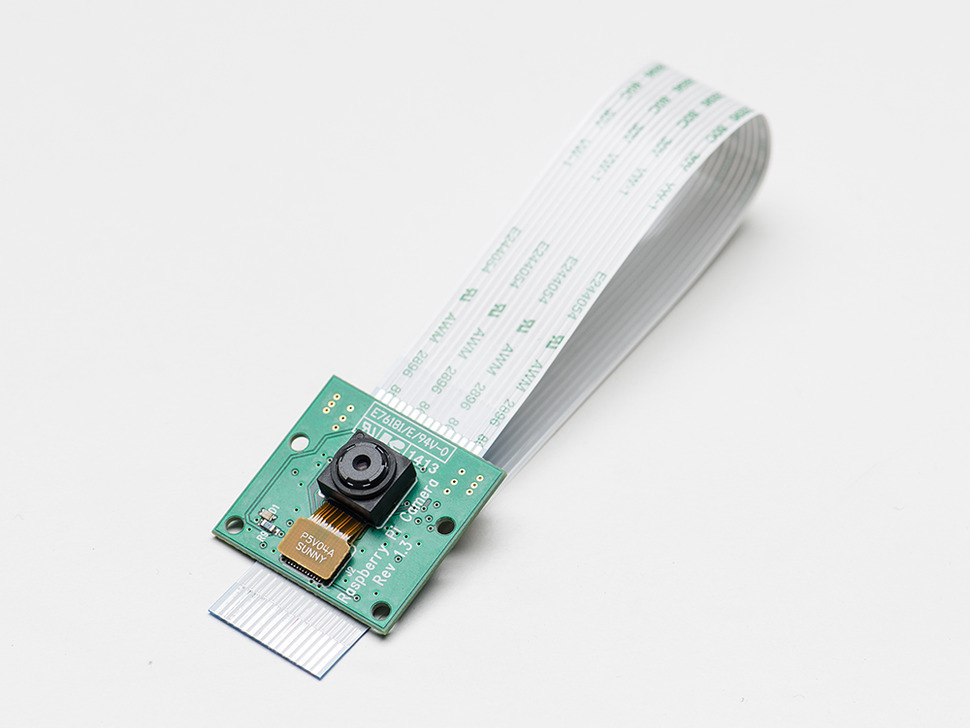
\includegraphics[scale=0.3]{imagenes/1367-01.jpg}


\caption{C\'amara Raspberry Pi}
\label{fig:came}
\end{figure}


\begin{itemize}
\item Batería de polímero de litio (Lipo): Es la fuente de poder usada para los motores y componentes electr\'onicos. La batería usada es de 11.1 voltios y 1 amperio. \cite{bateria}
\end{itemize}


\begin{figure}[hbtp]
\centering
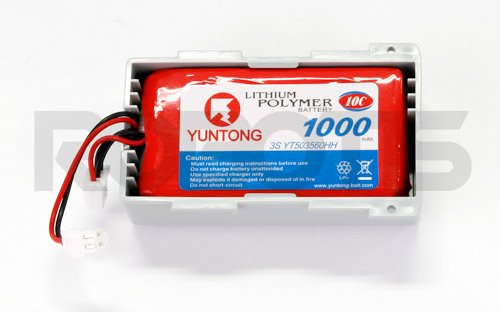
\includegraphics[scale=0.3]{imagenes/R-LIPOBAT.jpg}
\caption{Batería Lipo}
\label{bateria}
\end{figure}

\begin{itemize}
\item Circuito con regulador de 5v: Es un circuito diseñado y construido para este proyecto cuya finalidad es regular la entrada de la corriente. Por una de las salidas se expulsa 5v y por la otra se mantiene el mismo voltaje de entrada. 
\end{itemize}

%\begin{figure}[hbtp]
%\centering
%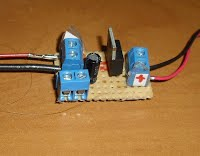
\includegraphics[scale=0.7]{imagenes/circuito.jpg}
%\caption{Lipo}
%\end{figure}

\label{subsection:construccion}
\subsection{Construcción}
Para la construcción del robot se utilizó el kit de piezas Bioloid Premium de marca Robotis el cual incluye motores Dynamixel Ax-12+, una tarjeta controladora CM-510, un sensor Gyro, un manual, entre otros elementos. El manual incluye las instrucciones de como armar varios modelos de humanoide, el utilizado en este proyecto es el tipo B, haciendo uso de 16 motores. En la figura ~\ref{fig:frontal} y ~\ref{fig:trasera1} se puede observar la estructura del robot que aparece en el manual del kit. 

\begin{figure}[hbtp]
\centering
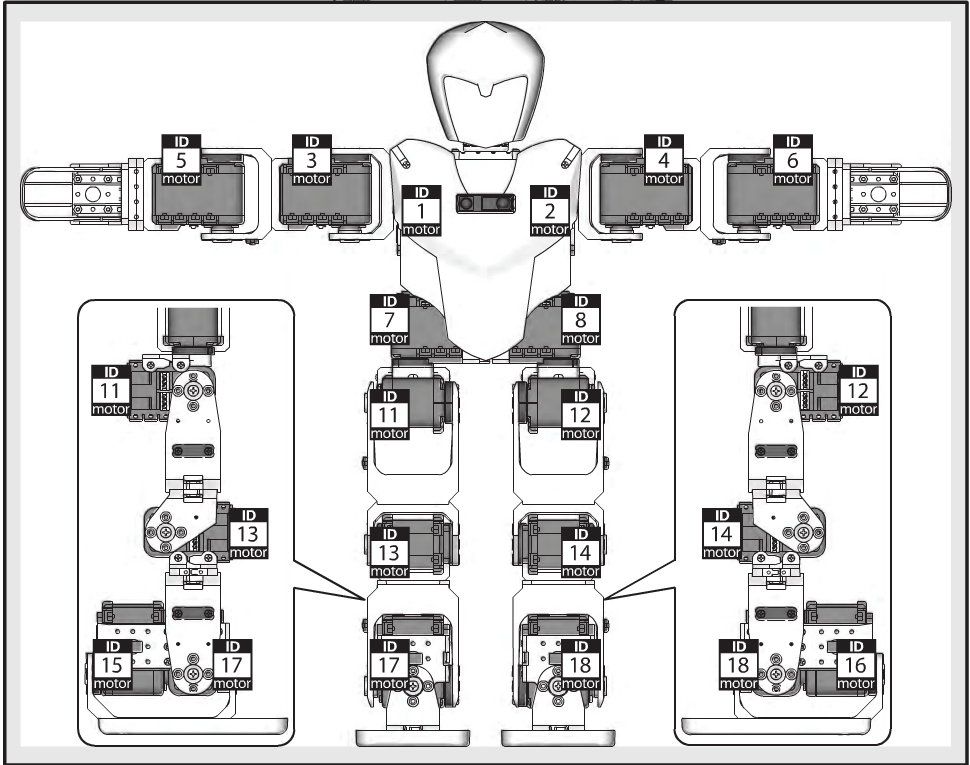
\includegraphics[scale=0.3]{imagenes/Robot.png}
\caption{Vista frontal del robot. Se puede apreciar la identificación ‘ID’ de cada motor Dynamixel Ax-12+. Nota: los motores 9 y 10 no se utilizan}
\label{fig:frontal}
\end{figure}

\begin{figure}[hbtp]
\centering
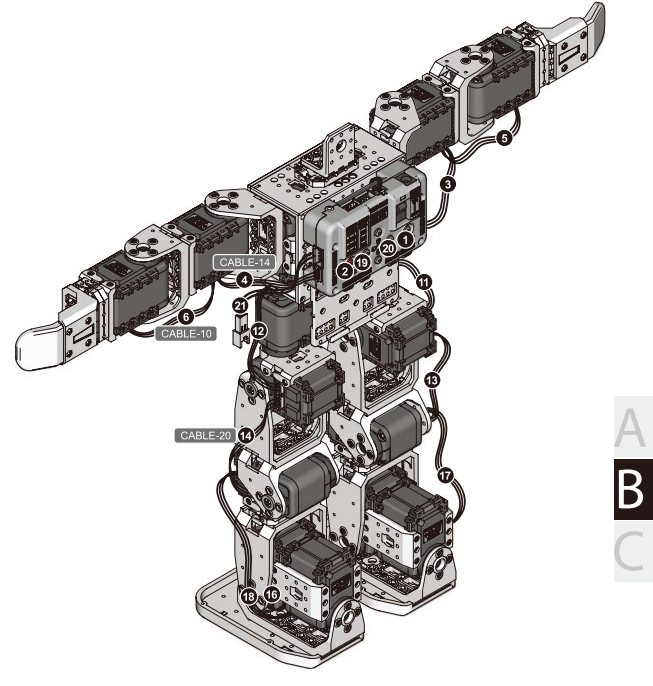
\includegraphics[scale=0.3]{imagenes/RobotTrasero.png}
\caption{Vista trasera del robot}
\label{fig:trasera1}
\end{figure}

El kit bioloid incluye una tarjeta controladora CM-510 la cual fue sustituida por la tarjeta controladora de software libre Arbotix. La utilización de la tarjeta Arbotix permite una mayor flexibilidad en el control de motores y la incorporación de una variedad de sensores no soportados por la tarjeta CM-510.
Además la tarjeta Arbotix posee mayor soporte y amplitud en la comunicación entre distintos dispositivos. 

En la figura ~\ref{fig:trasera2} se puede observar la estructura del robot con la Arbotix incorporada. En la parte interna del tronco del robot se sitúa el sensor Gyro.

\begin{figure}[hbtp]
\centering
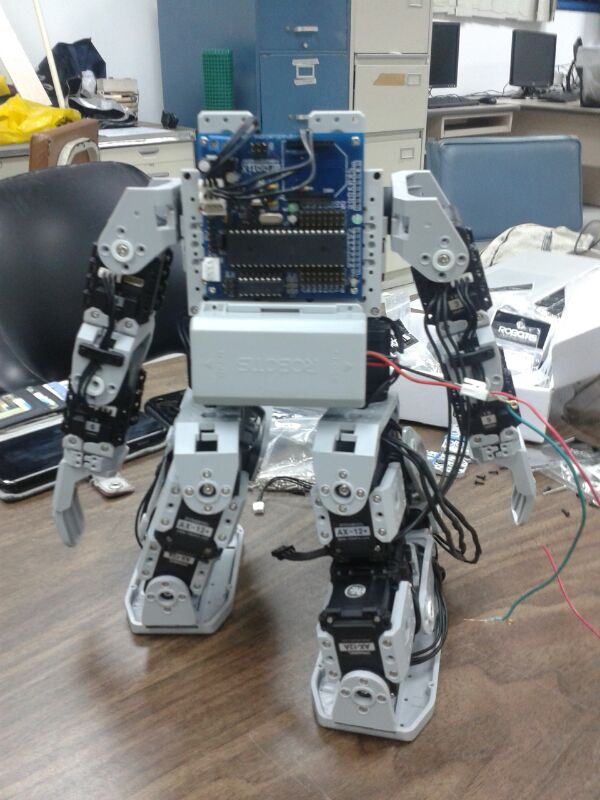
\includegraphics[scale=0.2]{imagenes/traseroDeJunny.jpg}
\caption{Vista trasera del robot con la Arbotix}
\label{fig:trasera2}
\end{figure}

\begin{figure}[hbtp]
\centering
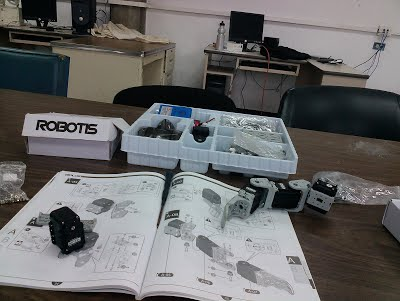
\includegraphics[scale=0.5]{imagenes/CIMG0225.jpg}
\caption{Manual de instrucciones y piezas del robot}
\end{figure}

Para el movimiento de la cámara se ha incorporado dos servomotores, uno para el movimiento horizontal y otro para el vertical. La conexión es pin a pin en los puertos especiales para ese tipo de motores (‘Hobby servos’) REF (ver figura ~\ref{fig:puertosHobby}). La cámara ha sido conectada a la Raspberry Pi en el puerto CSI (ver la figura ~\ref{fig:camACSI}). El resultado de estas tres piezas instaladas en el robot se puede apreciar en la figura ~\ref{fig:servosycam}.

\begin{figure}[hbtp]
\centering

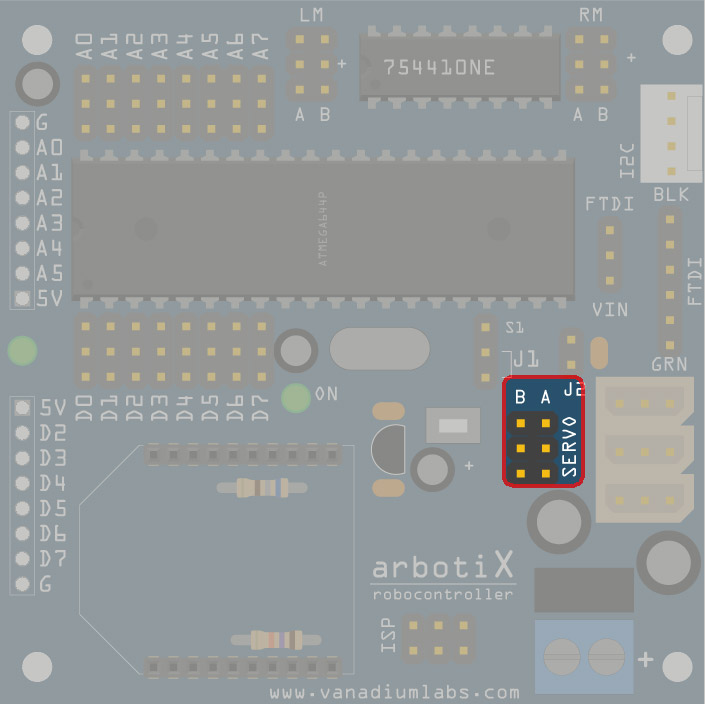
\includegraphics[scale=0.2]{imagenes/arbotix_hobby_servo.jpg}
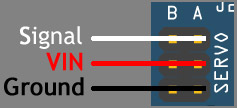
\includegraphics[scale=0.4]{imagenes/arbotix_hobbyservos_lines.jpg}
\caption{Ilustración de los puertos Hobby de la Arbotix}
\label{fig:puertosHobby}
\end{figure}

\begin{figure}[hbtp]
\centering
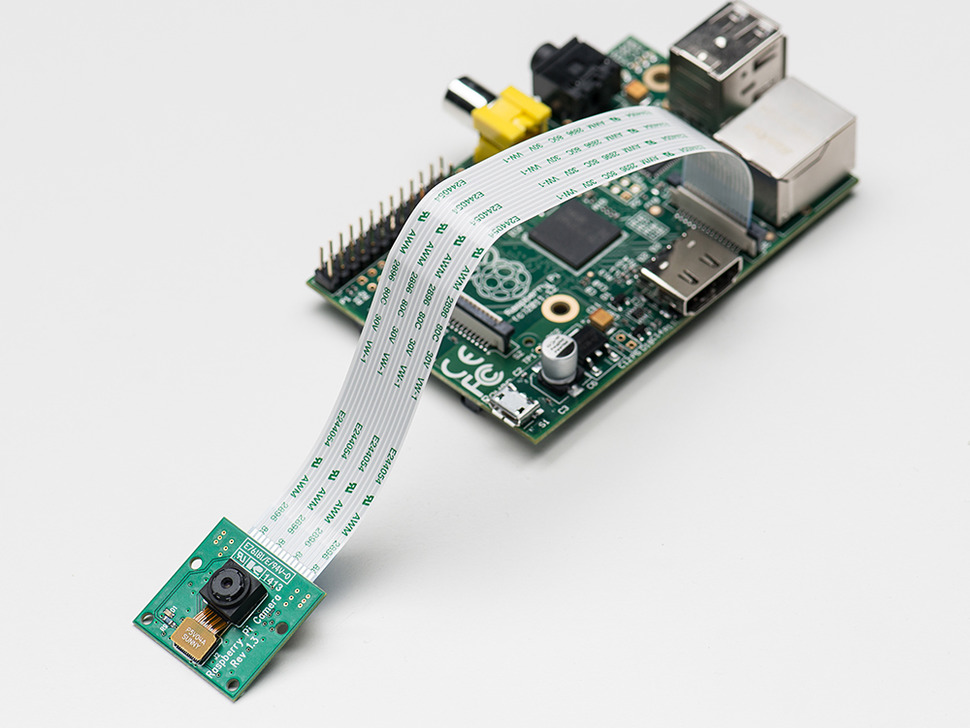
\includegraphics[scale=0.6]{imagenes/raspbCam.jpg}
\caption{C\'amara Raspberry Pi conectada al puerto CSI de la tarjeta}
\label{fig:camACSI}
\end{figure}
 
\begin{figure}[hbtp]
\centering
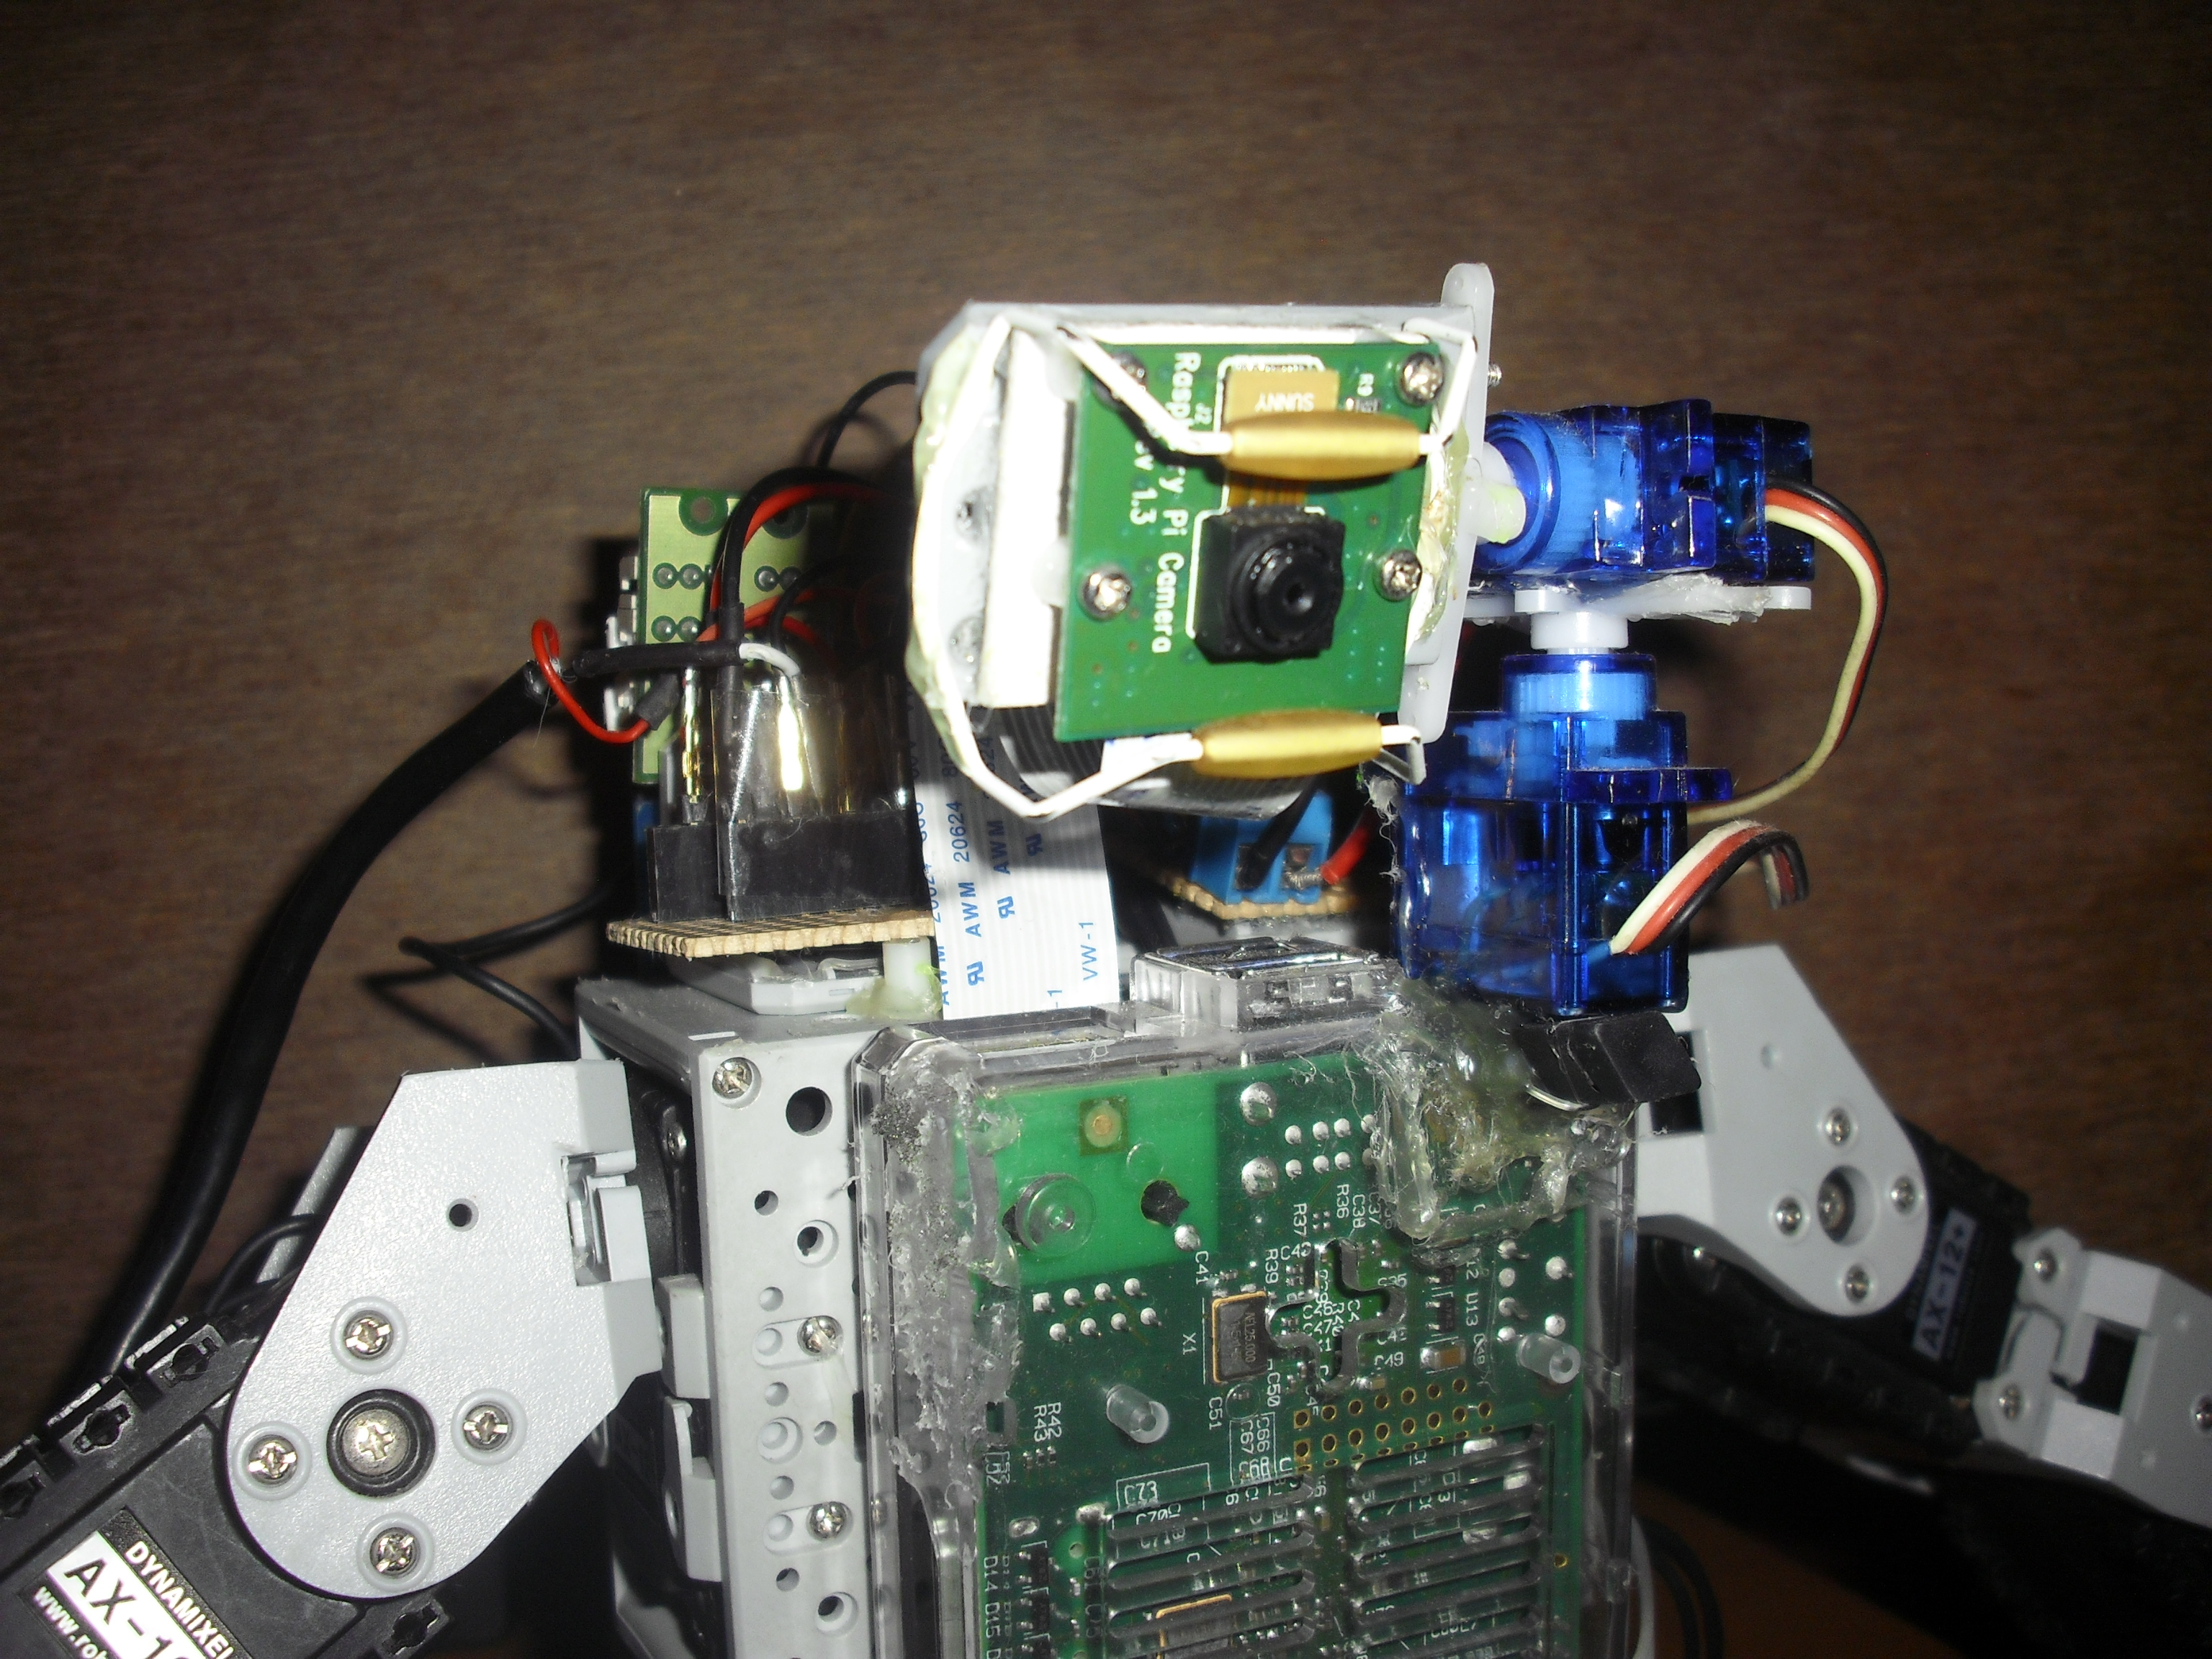
\includegraphics[scale=0.08]{imagenes/servosYcamara.JPG}
\caption{Vista delantera del robot con la cámara y servomotores instalados}
\label{fig:servosycam}
\end{figure}

Los motores Dynamixel se conectan a la controladora Arbotix por medio de los puertos bioloid de la tarjeta. La Arbotix s\'olo cuenta con tres puertos y el diseño del robot necesita cuatro series distintas 
una para cada extremidad por lo tanto cuatro puertos bioloid, se consideró la opción de unir dos extremidades pero ello implicaba limitaciones en el movimiento del robot por lo tanto se optó por agregar un expansor de puertos bioloid y así conectar cada extremidad en un puerto diferente. La forma en la que se ha conectado estos motores se ejemplifica en la figura ~\ref{fig:arbotixConectados}. 

\begin{figure}[hbtp]
\centering
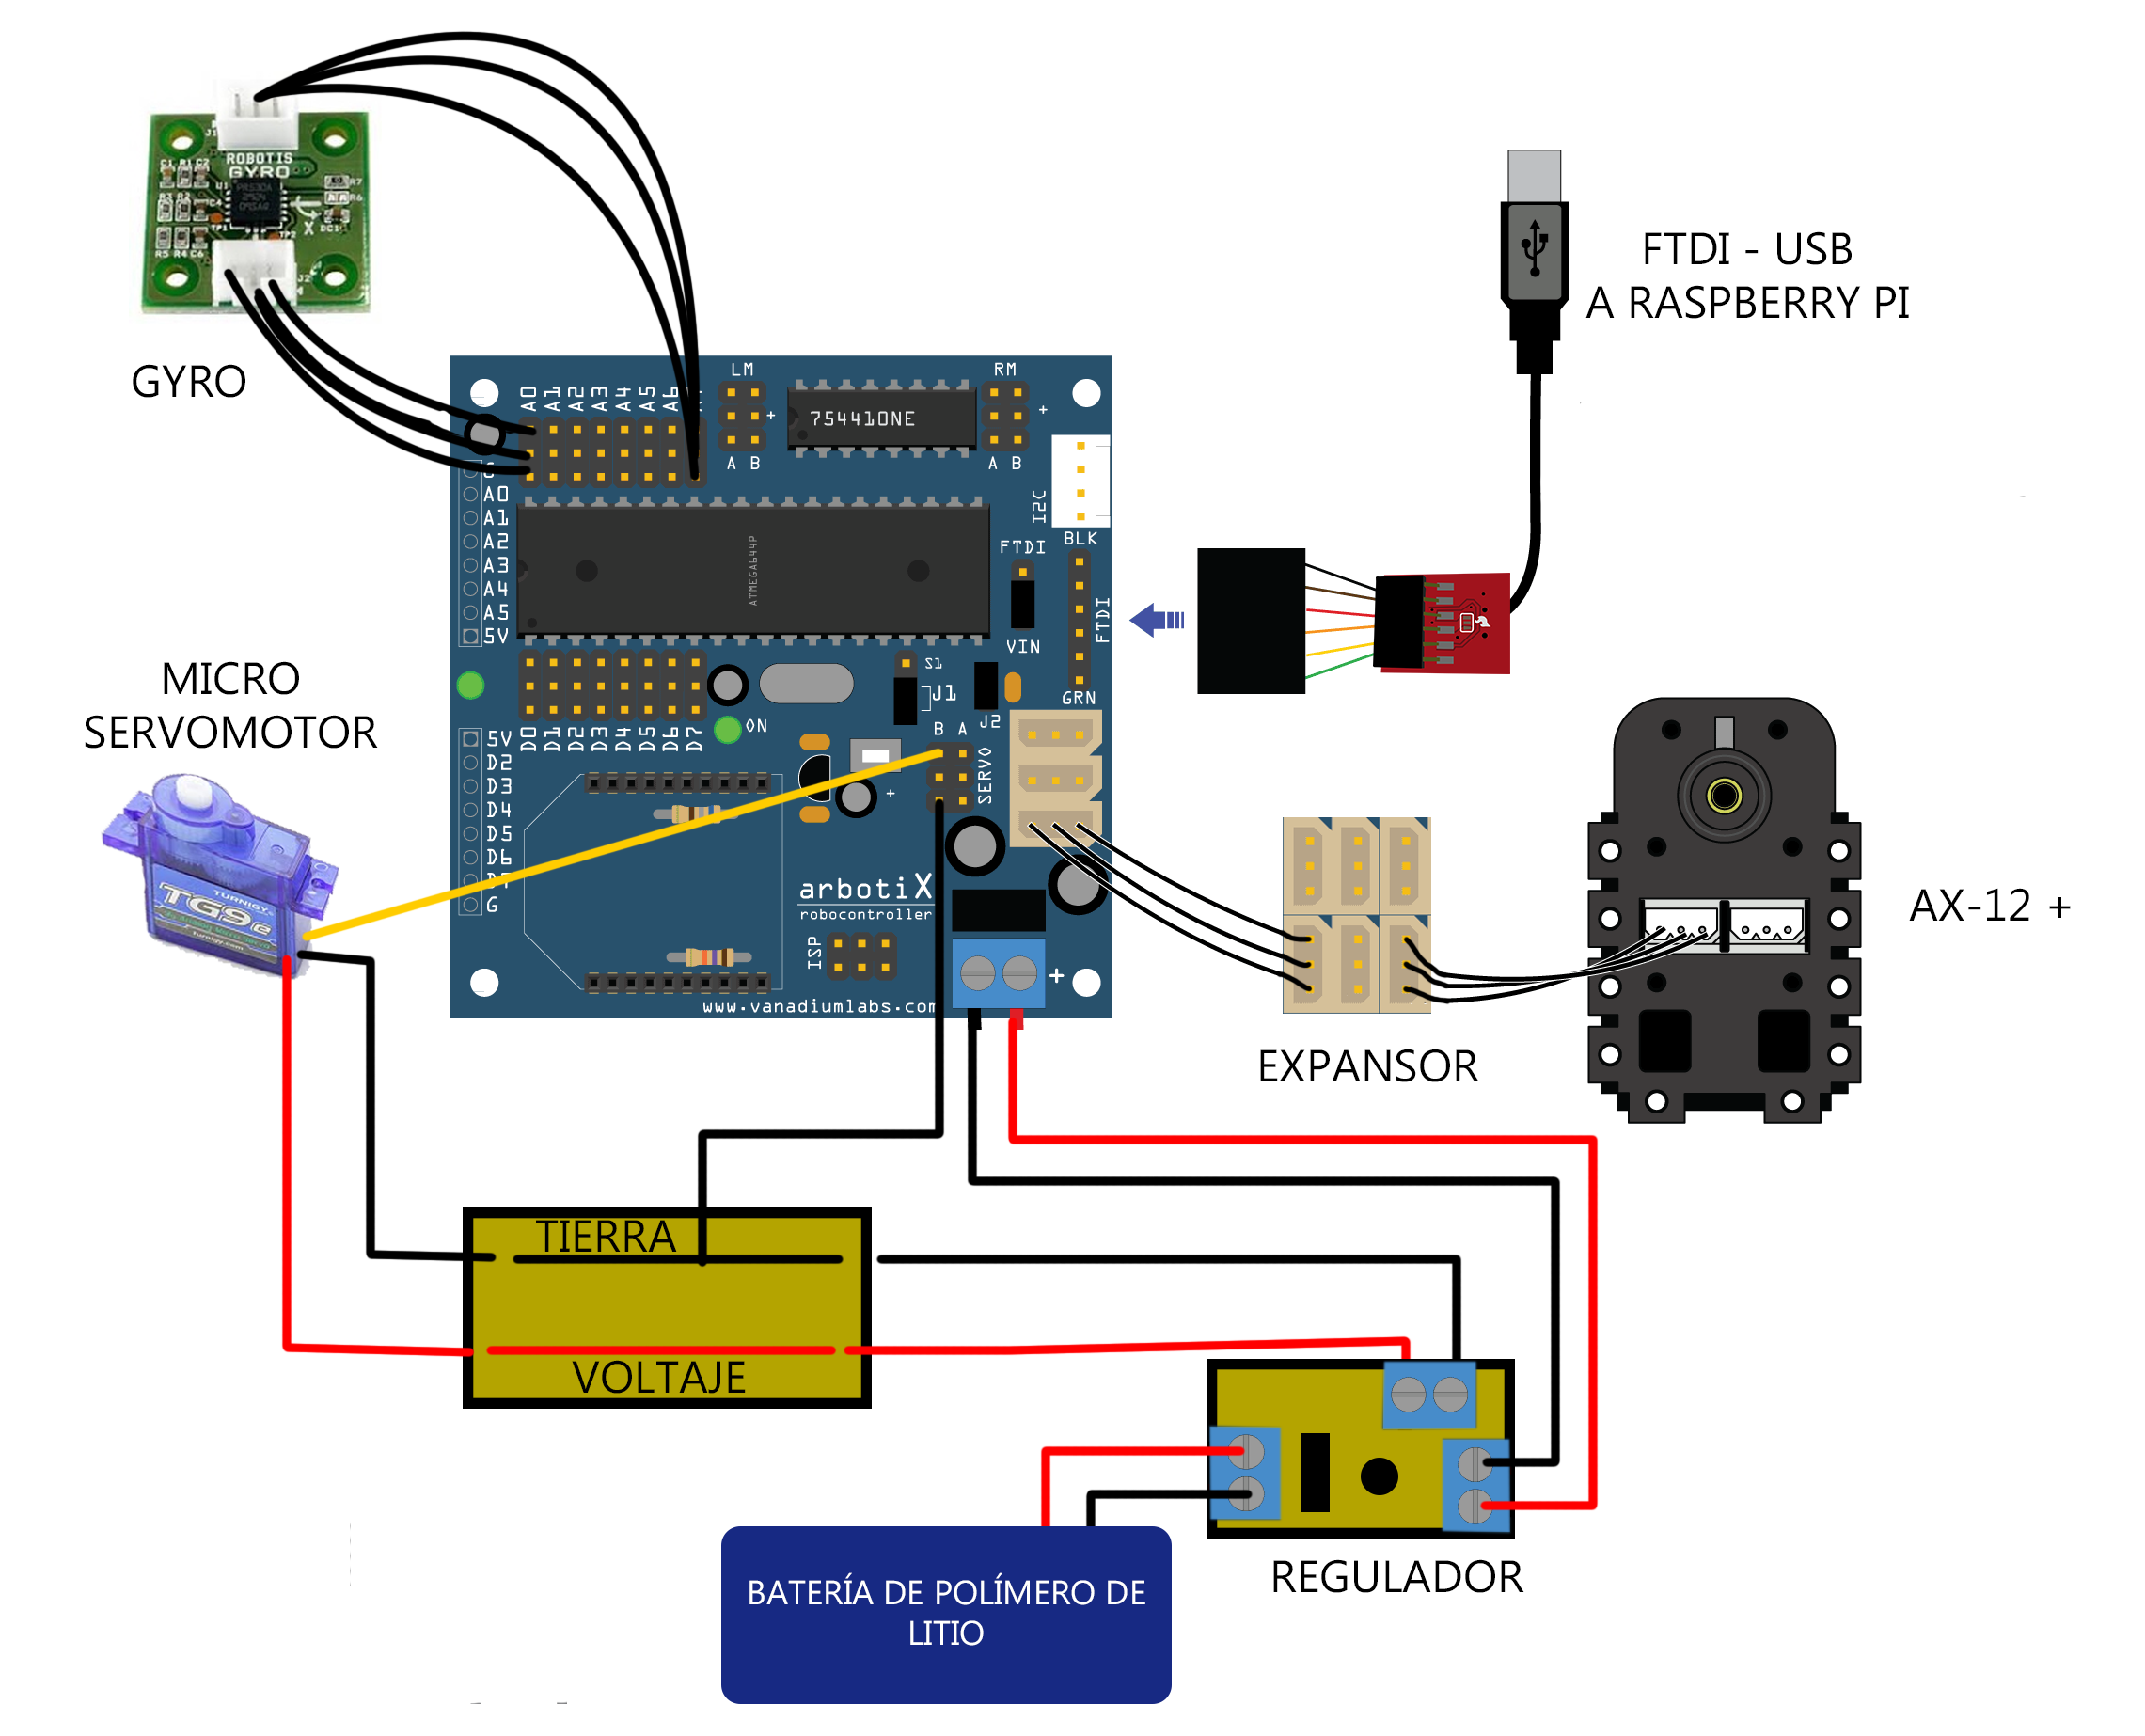
\includegraphics[scale=0.2]{imagenes/arbotix_servo.png}
\caption{Tarjeta controladora Arbotix y componentes conectados }
\label{fig:arbotixConectados}
\end{figure}

La comunicación de la tarjeta de Arbotix con la computadora, incluso con la Raspberry Pi, se realiza a través del puerto FTDI por medio un chip conectado como lo ilustra la figura ~\ref{fig:arbotixConectados}.

Como fuente de poder se utilizó una batería de polímero de litio de 11.1 V y 1 amp. Debido a que no todos los componentes poseen las mismas exigencias con respecto a voltaje y amperaje, se realizó un regulador (ver figura ~\ref{fig:circuito}) con  salida de 5 voltios para la tarjeta Raspberry Pi y los dos micro servomotores, con otra salida de 11.1 V para la tarjeta Arbotix que a su vez alimenta a los componentes conectados en ella (motores Dynamixel y Giroscopio). Si bien la tarjeta Arbotix posee un regulador interno de cinco voltios la opción de conectar todo a la salida de 5 V del regulador no era posible dado que los motores Dynamixel necesitan 11 voltios por lo tano se agregó la salida de 11.1 voltios.

\begin{figure}[hbtp]
\centering
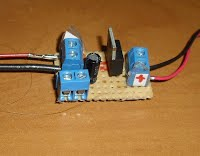
\includegraphics[scale=0.5]{imagenes/circuito.jpg}
\caption{Circuito con entrada de 11.1 V. Una salida de 5 V para los micro servomotores anal\'ogicos y tarjeta Raspberry Pi. Otra salida de 11 v para alimentar la controladora Arbotix.}
\label{fig:circuito}
\end{figure}



\section{Detección de la pelota}\label{chapter:deteccion}

La recopilación de información del medio ambiente, para detectar la posición de la pelota, se realiz\'o por medio de la cámara Raspberry Pi con el sistema operativo Raspian \cite{raspian}. Esta mini computadora y cámara constituyen una herramienta poderosa ya que permite capturar v\'ideos y fotos de alta definici\'on. Y como la Raspberry Pi cuenta con un procesador gr\'afico, este se encarga de manejar los datos de la cámara, aliviando la carga del procesador central \cite{raspCamArti}.

Además se ha decidido utilizar OpenCv \cite{opencv}, otra herramienta para procesar im\'agenes que se describe en la sección \ref{herramientasDetc}. Sin embargo los métodos de captura de OpenCV no funcionan con la c\'amara Raspberry Pi. En la secci\'on \ref{extraerImagen} se explica c\'omo se ha extra\'ido la imagen y en la secci\'on \ref{procesarImagen} se explica la forma en la que se ha procesado la imagen para hallar la posición de la pelota. 

\subsection{Herramientas software para la detecci\'on }\label{herramientasDetc}

Para extraer y procesar la imagen se utilizaron algunas librerias como apoyo. A continuación se presenta la descripción de la librería raspicam\_cv, usada para la extracción de la imagen y la descripción de la librería OpenCV, usada para la detección de la ubicación de la pelota.   

En visi\'on de computadoras existen varias liberias que apoyan y facilitan en procesamiento de im\'agenes, con herramientas de filtrado, transformaciones de im\'agenes, aprendizaje de m\'aquinas entre muchas m\'as. Dos ejemplos de ello son Processing \cite{processing} y OpenCv. Processing es un lenguaje de programaci\'on que esta enfocado para iniciar a personas no programadoras en el \'area, por lo tanto explota la retroalimentaci\'on visual para atraer al usuario, posee herramientas de filtrado, de transformaci\'on de im\'agenes y muchas otras .
Por otro lado OpenCv (Open Source Computer Vision Library) es una librería de visión de computadoras y aprendizaje de máquinas de código abierto. Ha sido diseñada para acelerar el uso de la percepción de m\'aquinas y para proveer una estructura común en las aplicaciones de visión de computadoras \cite{opencv}. La decisi\'on de utilizar OpenCv se basa en su mayor amplitud de herramientas ofrecidas, un filtrado de im\'agenes mas amplio, un mayor control en el manejo de las im\'agenes y sus transformaciones.

Raspicam\_cv es una librería que permite obtener im\'agenes de la cámara Raspberry Pi en una estructura de datos compatible con OpenCV \cite{emilV}.

\subsection{Obtenci\'on de la imagen}\label{extraerImagen}

%<<<<<<< HEAD
%Dentro de las librerías oficiales para la cámara Raspberry Pi s\'olo se encuentran implemetadas en el lenguaje interpretado python y algunas aplicaciones para la línea de comandos de linux. Para utilizar la cámara con OpenCV en el lenguaje compilado \gls{C++} se requirió realizar una búsqueda de librerias alternas a las oficiales. Una primera solución se encontró en el blog de \cite{pierreR}, en donde explica que los métodos de captura de video de OpenCV no funcionan de manera nativa con el m\'odulo de la cámara de la Raspberry Pi (por ejemplo el método cvCapture). Para lograr extraer la imagen se basó en el código abierto de las aplicaciones raspivid y raspistill. Ha modificado el código para usar el buffer de la cámara y así obtener un objeto compatible con OpenCV. 
%raspicam\_cv es la librer\'ia utilizada en el proyecto que del c\'odigo ha sido moficicada convirtiendola una librer\'a por \cite{emilV}.
%=======
Dentro de las librerías oficiales para la cámara Raspberry Pi s\'olo se encuentran aquellas implemetadas en el lenguaje interpretado python y algunas aplicaciones para la línea de comandos de linux. Los métodos de captura de video de OpenCV no funcionan de manera nativa con el m\'odulo de la cámara de la Raspberry Pi (por ejemplo el método cvCapture). Para utilizar la cámara con OpenCV en el lenguaje compilado \gls{C++} se requirió realizar una búsqueda de librerias alternas a las oficiales. Se hayó una primera solución modificando las aplicaciones \gls{raspivid} y \gls{raspistill} para lograr extraer la imagen del buffer de la cámara y así obtener un objeto compatible con OpenCV \cite{pierreR}. Sin embargo era poco práctico porque se debía incluir todo el código en el proyecto y compilarlo unido. Luego se encontró que en base en ese trabajo, se había construido una librería de código abierto. Esta librería se llama raspicam\_cv y es es la que ha sido utilizada en este proyecto \cite{emilV}.

%Una primera solución se encontró en el blog de , en donde explica que 

\subsection{Procesamiento de la imagen}\label{procesarImagen}

Con ayuda de la librería OpenCv, en \gls{C++}, se filtra y procesa la imagen para obtener la posición de la pelota en un momento dado y de forma autónoma. 

Para encontrar la ubicación de la pelota  se ha decidido aplicar detección por segmentación de regiones, esta técnica consiste en filtrar la imagen por segmentaci\'on de color, por ello es importante que el color de la pelota no se repita en el ambiente y así poder obtener su posición dentro de la imagen. Esta t\'ecnica de segmentaci\'on es la m\'as com\'un en detecci\'on de objetos y muy utilizada en competencias de rob\'otica. La t\'ecnica de detecci\'on por  formas fue puesta a prueba tambi\'en pero con la misma no se pudo obtener resultados pr\'acticos ya que no lograba detectar correctamente la pelota. Vale la pena acotar que la detecci\'on por formas aplicada no implementaba ning\'un tipo de aprendizaje de m\'aquinas.

%La imagen es captada en el modelo de color \gls{RGB} y se transforma al \gls{HSV}. Luego se aplica la función inRange de OpenCv para obtener una imagen en blanco y negro, en donde se identifica con blanco la zona con el color de la pelota y el resto de la imagen en negro. En el procesamiento de im\'agenes y visi\'on de computaci\'on se trabaja con las im\'genes en escala de grises pues disminuye el tiempo en procesar datos que poseen informaci\'on inutil y aumenta la eficiencia.
%=======
La imagen es captada en el modelo de color \gls{RGB} y se transforma al \gls{HSV}. Luego se aplica la función inRange de OpenCv para obtener una imagen binaria, en donde se identifica con blanco la zona con el color de la pelota y el resto de la imagen en negro. En el procesamiento de im\'agenes y visi\'on de computaci\'on se trabaja con las im\'genes en escala de grises, pues disminuye el tiempo en procesar datos que poseen informaci\'on inutil y aumenta la eficiencia.

Para disminuir el ruido y los posibles elementos aislados que pueda tener la imagen con la que se está trabajando se han aplicado los filtros o transformaciones de morfología en apertura y morfología en clausura de la librería Opencv, basadas en las operaciones básicas de dilatación y erosión. La morfología en apertura es una transformación que consiste en aplicar la operación de erosión seguido de la operación de dilatación. La morfología de clausura es una transformación que aplica la dilatación seguido de la erosión.

De esta forma se logró ubicar la pelota con la cámara Raspberry Pi en el 100\% de las pruebas realizadas, que se describen en el cap\'itulo \ref{chapter:resultados}.



\section{Busqueda y Pateo}\label{chapter:busqueda}

Para poder buscar y patear la pelota, además de tener la capacidad para detectarla (como se explicó en el capítulo anterior), debe ser capaz de moverse en su entorno, tener una representación del mundo que lo ayude a orientarse y planificar una estrategia para elegir el conjunto de movimientos que lo lleven a acercarse a la pelota. 

En esta sección se explica el desarrollo de las actividades que han sido necesarias para ejecutar la búsqueda y pateo de la pelota, con excepción de la estrategia de toma de acciones, que se explicará en la siguiente sección.

Primero, en la sección (herramientas) se da una breve descripción de las herramientas de software que apoyaron las tareas de búsqueda y pateo. En la sección (movimientos) se explica cual fue el conjunto de movimientos creados para el esqueleto del robot.

El sensor principal de Junny, es el observador de su ambiente, la c\'amara. En la secci\'on (movCamara) se explica las posiciones que puede adoptar. Luego en la seccion (mundo) se explica la manera en la que Junny organiza la representaci\'on visual que capta del mundo, que se ha decidido dividir por estados.

Debido a que el movimiento del robot se controla desde la tarjeta Arbotix y la detecci\'on de la pelota se hace desde la Raspberry Pi, se debi\'o establecer la comunicaci\'on entre ambas tarjetas. Este proceso se explica en la secci\'on (comunicacion).

Una vez con la representaci\'on del mundo en estados, los movimientos programados y la comunicaci\'on de las tarjetas, solo faltaria decidir que acci\'on tomar en cada estado. Esta estrategia se explica en la siguiente secci\'on (numero de la seccion).        

%Como se mencion\'o anteriormente el robot debe buscar y patear una pelota de tamaño de una pelota de tennis y ya se ha descrito las caracter\'isticas f\'isicas y de software que utiliza el robot, esta secci\'n se enfoca en el comportamiento que describe a este robot.
%Para ello primero se especifica la serie de movimientos implementados y el comportamiento que lo representa.
 
\subsection{Herramientas software para la busqueda de la pelota } \label{chapter:busqueda}

Decir mas o menos para que usamos cada herramienta, breve. 

\begin{itemize}
\item Pypose: Software especializado en el control de los servomotores Dynamixel Ax-12. Una de las más importantes características es que, luego de haber fijado a mano las posiciones de los motores, permite la lectura simultánea de esas posiciones para captar la pose del robot. Con esta herramienta es posible formar una secuencia de poses que generen un movimiento, por ejemplo, caminar \cite{pypose}. 

\item IDE Arduino: Es un entorno de desarrollo para escribir y cargar código en la tarjeta Arduino. Otras tarjetas con microcontroladores AVR también son compatibles, como la ArbotiX. El lenguaje de programación del IDE de Arduino es una implementación de Wiring el cual esta basado en Processing \cite{arduino}.  

\item ROS: ROS (Robot Operating System) es un framework que proporciona bibliotecas y herramientas para ayudar a los desarrolladores de software a crear aplicaciones robóticas. Proporciona abstracción de hardware,  de dispositivos, bibliotecas, visualizadores, paso de mensajes, gestión de paquetes y más. ROS se encuentra bajo licencia de código abierto, la licencia BSD.

\end{itemize}

\subsection{Comportamiento}

Debupa es un robot humanoide implemetado de forma autonoma e inteligente que sigue un comportamiento bajo el paradigma h\'ibrido (secci\'on 2 ). El sensor principal (c\'amara ) es el observador del mundo, que posee una serie de movimentos determinados (secci\'on REF) con los cuales escanea el mundo y combinados con la serie de movimiemtos del esqueleto es capaz de encontrar la pelota. Al determinar la posici\'on de la pelota Debupa logr\'o aprender (secci\'on APRENDIZAJE) la mejor acci\'on a relizar para estar mas cerca de ella y al llegar poder patearla.

\subsection{Movimiento del esqueleto}
\label{esqueleto}
El robot debe desplazarse para poder patear la pelota por ello se describen y definen los movimientos del esqueleto que se fueron utilizados.

Con fines explicativos, en este proyecto, la palabra ''pose" se referire a la posición específica de los 16 motores que constituyen el esqueleto del robot. Un conjunto de poses ejecutadas en secuencia se denominará ''acción de movimiento".


Las acciones de movimiento establecidas son:


\begin{itemize}
 \item {Caminar hacia adelante}
 \item {Caminar hacia adelante}
 \item {Caminar hacia adelante}
 \item {Girar a la izquierda}
 \item {Girar a la izquierda} 
 \item {Girar a la derecha}
 \item {Girar a la derecha}	 
 \item {Levantarse cuando ha caído boca abajo}
 \item {Levantarse cuando ha caído boca arriba}
 \item {Patear con la pierna derecha }
 \item {Patear con la pierna izquierda}
 
\end{itemize}

Existen también dos acciones de movimiento que no se encuentran relacionadas con la posición de los motores del esqueleto del robot sino a la posición de los motores que controlan la posición de la cámara. Estas se explicarán en la sección de movimiento de la cámara.

Las poses han sido fijadas a través de la tarjeta controladora Arbotix y el software Pypose. De esta manera se ha fijado y guardado un conjunto de poses para cada acción de movimiento. Estas acciones de movimientos son utilizadas en el programa, en lenguaje Wiring, a ser ejecutado en Arbotix. La programación en Arbotix se ha realizado bajo el ambiente del IDE de Arduino. 


\subsection{Movimiento de la cámara}
La cámara ha sido instalada sobre dos micro servomotores analógicos, otorgándole dos grados de libertad. El servomotor ubicado en la parte inferior se encarga del movimiento horizontal y el superior del movimiento vertical. Las acciones de movimiento relacionadas con el movimiento de la cámara se reduce a 6 posiciones fijas en la figura se puede ver ~\ref{fig:posicionesCam} cuya distribución obedece al objetivo de que la cámara obtenga una amplia visión, sin dejar espacios no visibles. 



\begin{figure}[hbtp]
\label{posicionesCam}
\centering
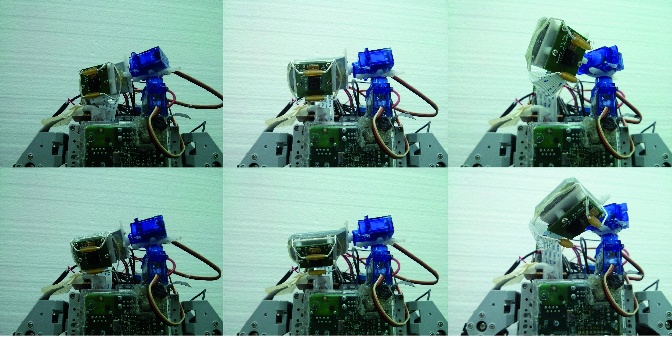
\includegraphics[scale=0.5]{imagenes/Pantallazo.png}
\caption{Posiciones de la cámara }
\end{figure}

Estos motores se controlan desde la Arbotix usando la librería HServo. Esta librería solo puede ser usada para los motores conectados en los puertos Hobby A y B (pines 12 y 13) (ver la figura ~\ref{fig:puertosHobby}). Brinda la ventaja de un control más preciso, evitando que los motores tengan una vibración ya que los pulsos son generados por temporizadores de hardware. 

\subsection{Representacion del mundo en estados}

El hecho de  que la cámara tenga dos grados de libertad para moverse es una gran ventaja, ya que se puede obtener un mayor rango de visión. Debupa puede mirar hacia la derecha o izquierda sin tener que mover sus piernas, también puede mirar hacia abajo para verificar que la pelota esté en sus pies, para patear, o hacia arriba para ubicar la pelota a mayor distancia.

La estrategia para poder llegar a la pelota consiste en mover la posición de la cámara hasta encontrar la pelota, en caso de encontrarla, dependiendo de su ubicación dentro de la imagen y la posición de la cámara se toma una acción diferente, en caso de no encontrarla el robot gira con los pies para cambiar su orientación física e iniciar nuevamente el movimiento de la cámara para hallar la pelota. Cuando se tiene la pelota en una posición cercana a los pies se realiza la acción de patear. 

En la siguiente sección se explicará la manera en la que se dividen las regiones en una imagen para determinar la acción a tomar y el orden en el que se mueve la cámara.

Debupa debe tomar una acción diferente dependiendo de la posición de la cámara y de la pelota en la imagen. Sin embargo esto genera una gran cantidad de estados, por lo cual se ha decidido discretizarlos de la siguiente manera:  

La cámara tiene 6 (2x3) posibles posiciones. La visión horizontal abarca 3 cuadros, aproximadamente 160 grados, por razones de la estructura del robot no se le ha podido agregar un rango más grande. La visión vertical abarca 2 cuadros, llega a captar la imagen desde sus pies hasta más de 2 metros hacia adelante.

Desde cada posición de la cámara se obtiene una imagen. Las imagenes de la cámara en posición central, y en posicion central inferior son las más importantes y prioritarias, pues si la pelota se detecta en ellas significa que el robot está cerca de poder patearla. Estas dos imagenes se dividen en subregiones, para tener mayor precisión en las acciones que Debupa deba tomar. Una representación sencilla de la discretizacion del ambiente se puede apreciar en la figura ~\ref{fig:divisionCam}. El área de pateo son las regiones 15 y 16. Por ejemplo, en el cuadro del central inferior, cuando la pelota se encuentra del lado derecho de la pantalla (region 13 o 17) el robot debe girar a la derecha para situarse de frente a la pelota.

Las imágenes capturadas desde cada posición de la cámara se solapan para evitar perder de vista a la pelota. 

Las acciones específicas a tomar según el estado en que se encuentre la pelota se realizan por medio de lo aprendido en el entrenamiento realizado con apredizaje por reforzamiento. Los detalles de este aprendizaje se describen en la seccion 3.4.
%A continuación se especifica la acción a tomar en cada region: 
 
%Girar a la Izquierda: Debupa debe girar a la izquierda cuando la pelota se encuentre en alguna de las siguientes regiones: 1, 4, 10, 5, 11, 14.

%Girar a la Derecha: debe girar a la derecha cuando la pelota se ubique en alguna de las siguientes regiones: 7, 13, 17, 3, 9, 18. 

%Caminar hacia adelante: cuando la pelota se ubique en alguna de las siguientes regiones: 12, 6, 2.

%Patear con la pierna izquierda: cuando la pelota se encuentre en la región 15.

%Patear con la pierna derecha: cuando la pelota se encuentre en la región 16.

\begin{figure}[hbtp]

\centering
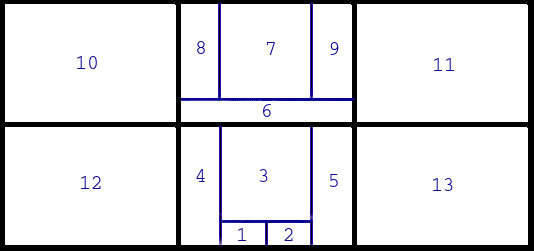
\includegraphics[scale=0.5]{imagenes/Regiones.jpg}
\caption{Campo de visión del robot con el número de cada región. Cada cuadro blanco demarcado con líneas negras representa la posición de la cámara. La región de pateo de la pelota se encuentra en los cuadros 15 y 16 }
\label{divisionCam}
\end{figure}


\subsection{Comunicación Arbotix - Raspberry (ROS)}

La Raspberry Pi procesa la información de la cámara y la Arbotix controla los actuadores. Para coordinar los movimientos del robot según la posición de la pelota se estableció una forma de comunicación entre ambas tarjetas. 

Se ha establecido la Arbotix como servidor de peticiones y a la Raspberry Pi como cliente. Dentro de la Raspberry Pi se ejecuta el proceso de decidir qué acción debe tomar el robot. Una vez determinada la acción se envía la petición a la Arbotix para que esta la ejecute. Este proceso es bidireccional y síncrono, es decir, la Raspberry envía la petición y se bloquea hasta que la Arbotix retorne la respuesta de su culminación.  

Para la implementación de la comunicación se ha usado ROS con su versión Hydro y se ha utilizado la interfaz de comunicación basada en servicios que no es más que un método de comunicación basado en el paradigma de resquest / reply con el concepto de maestro esclavo. REF



\section{Aprendizaje}\label{aprendizaje}
En aprendizaje de m\'aquinas el aprendizaje por reforzamiento es una forma de plantear el problema de inteligencia completamente distinta a el aprendizaje supervisado o no supervisado que generalmente esta basado en ejemplos y un par entrada/salida, el objetivo del agente es aprender la funci\'on que haya producido esos pares. Sin embargo no siempre existe un supervisor que pueda verificar los resultados otorgados.
Existen ambientes en la vida real donde al agente no se le proporciona ni el supervisor ni los ejemplos, en donde se comienza sin contar con un modelo del ambiente o una funci\'on de utilidad. En estos casos la aplicaci\'on del aprendizaje por reforzamiento es la mas indicada \cite{peterAndNorvig}.

La t\'ecnica de refuerzo es aplicada en la vida diaria constantemente pues esta basada en comportamientos, es la forma en que se entrena a una mascota, es la manera en que un bebe logra aprender a sujetar objetos, esos son ejemplos de los muchos en los que en la realidad aparece esta t\'ecnica de aprendizaje.

Cuando es aplicada a inteligencia artificial las bases son las mismas, obviamente a un robot no se le podr\'a dar una galleta literalmente como premio de su buena acci\'on o quitarle la televisi\'on como castigo.
 
Existen varias estrategias que permiten otorgar recompensas positivas o negativas pertinentes al un agente en este caso un robot, con ellas ir moldealdo el comportamiento a uno que se considere correcto.

Un algoritmo para aprender por reforzamiento es aprendizaje-Q, que es el utilizado para que Junny aprenda a acercarse a la pelota.
 
%En el área de inteligencia artificial, asociada a robótica, existen variadas técnicas que permiten que un robot pueda aprender a realizar alguna tarea. En este caso particular se utiliz\'o la técnica de aprendizaje por reforzamiento que consiste en dar recompensas positivas o negativas dependiendo del desempeño del robot.


Según \cite{Mitchell} todo aprendizaje se define por la realización de una tarea $T$, cuyo desempeño medido por $D$, mejora con la experiencia $E$. En la investigación presente la tarea $T$ es aprender cuál es el mejor conjunto de ``acciones de movimiento" que se debe tomar con la finalidad de acercarse a la pelota. La experiencia $E$ se da a través un conjunto de pruebas, en las que Junny debe buscar la pelota y posicionarse frente a ella. El desempeño $D$ se mide con respecto a si el robot logra posicionar la pelota en el área de pateo y cuántas acciones de movimiento son necesarias para lograrlo.

Como existe incertidumbre con respecto a la dinámica del ambiente (esto es, no se conoce la función $\delta(s,a)$, definida en la subsección \ref{subsec:Qlearning} se utilizó el modelo de aprendizaje Q-learning \cite{Mitchell}, el cual permite mejorar el desempeño de la tarea definida en base a la experiencia de cada prueba. A continuación se presenta y describe la configuración de las caracter\'isticas particulares del aprendizaje utilizado para este proyecto.

\subsection{Modelo del problema}

El algoritmo para Q-learning se adapta a problemas configurados como procesos de decisión Markovianos (MDP). En este tipo de problemas el resultado de aplicar una acción en un estado particular depende solo de ese estado y esa acción, no de las acciones del pasado. 

En un MDP, un agente representa su mundo a través de un conjunto de estados y tiene un conjunto de acciones que puede ejecutar. Cada vez que el agente identifica el estado en el que se encuentra y escoge una acción para tomar, dependiendo del resultado, este recibe una recompensa determinada.

En la sección \ref{estados} se define el conjunto de estados que conforman el mundo de Junny. En la secci\'on \ref{sec:acciones} se dan a conocer las posibles acciones definidas y en la secci\'on \ref{recompensas} se define la ecuaci\'on para calcular las recompensas.   

\subsubsection{Estados}\label{estados}

De forma general se puede decir que los estados se encuentran definidos en función de la posición de la pelota con respecto al robot. En la sección \ref{mundo} se ha explicado la manera en la que se representa el mundo en base a 13 regiones en las que se puede encontrar la pelota. Para el aprendizaje se ha decidido ampliar el número de regiones para afinar y mejorar el tiempo en el que se llega a la pelota. Estas regiones se muestran el la figura ~\ref{fig:estados2}.

Cada región en la que se pueda detectar la pelota es un estado diferente. Por lo tanto se generan 18 estados, 17 de ellos se corresponden con la detección de la pelota en cada una de las regiones que se muestran en la imagen ~\ref{fig:estados2} y el estado número 18 representa la ocasión en la que no se logra ubicar la pelota en ninguna de las regiones.  

\begin{figure}[hbtp]
\centering
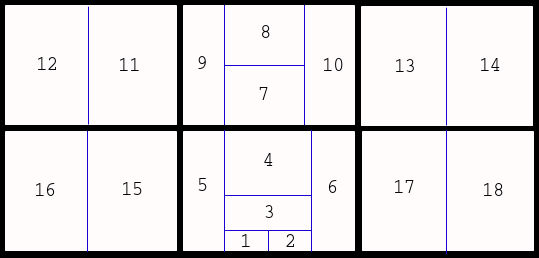
\includegraphics[scale=0.5]{imagenes/Regiones2.jpg}
\caption{Estados definidos seg\'un la región en la que se detecta la pelota}
\label{fig:estados2}
\end{figure}


\subsubsection{Acciones}\label{sec:acciones}

Las posibles acciones a realizar son un subconjunto de las acciones de movimiento definidas en la sección \ref{esqueleto}. Además se agregaron otras acciones para mejorar el desempeño en la búsqueda de la pelota. Las acciones disponibles son:

\begin{itemize}
\item {Caminar un paso hacia adelante }
\item {Caminar dos pasos hacia adelante }
\item {Caminar cuatro pasos hacia adelante}
\item {Girar a la izquierda}
\item {Girar doble a la izquierda} 
\item {Girar a la derecha }
\item {Girar doble a la derecha}
\label{item:todaslasacciones}
\end{itemize}
%%%%%%%%%%%%%%%%%%%%%%%%%%%%%%% NO SE SI PONER ESTO O NO %%%%%%%%%%%%%%%%%%%%%%%55
%Las acciones poseen una distancia recorrida por cada una, un paso hacia adelante desplazada 2.5 cm, dos pasos hacia adelante 4.8 cm , cuatro pasos recorre 9.9 cm , en cuanto a los giros simples la distancia es de 3cm y los giros dobles de 6 cm.
\subsubsection{Recompensas}\label{recompensas}

La recompensa, que puede ser positiva o negativa, se otorga a un par $(s,a)$, en donde $s$ es un estado y $a$ es una acci\'on. Se calcula en base a que tanto el robot se acerca a la pelota cuando en el estado $s$ se toma la acci\'on $a$. Es decir, las recompensas se definen en base a la distancia recorrida, con respecto a la pelota, cuando se toma una acci\'on.  

La distancia de una región con respecto al área de pateo, se define con la función $d: r \rightarrow y$ con $r \in \{1,2,3 ...18\}$ y $y \in \{1,2,3 ...10\}$. En donde $r$ es el número de la región y $y$ es la distancia de la región con respecto al \'area de pateo. Se asign\'o una distancia a cada regi\'on como se muestra en la figura ~\ref{fig:distancias}. El valor 1 se le asigna a las regiones m\'as cercanas al robot (zonas de pateo), $d(1)= 1$ y $d(2)=1$; el valor 10, a las regiones m\'as lejanas (regiones 12 y 14). Adicionalmente se define la distancia de la región 18 como $d(18)=10$. 
     
\begin{figure}[hbtp]
\centering
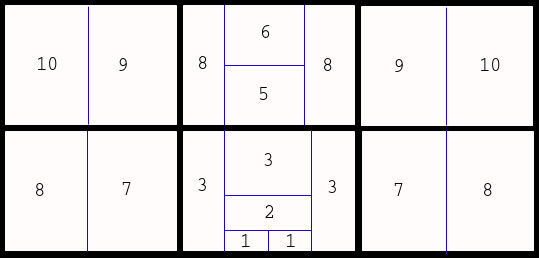
\includegraphics[scale=0.5]{imagenes/Distancias2.jpg}
\caption{Distancias relativas de la pelota establecidas para otorgar la recompensa.}
\label{fig:distancias}
\end{figure}

Junny gana una recompensa positiva cuando, con una acción, la pelota pasa de una región de mayor valor (lejana) a una de menor valor (más cercana). Si la pelota se mantiene en la misma región obtiene recompensa 0. De lo contrario obtiene una recompensa negativa. La ecuación se define como:



\begin{equation}
R(s,a,s') = \dfrac{d(s) - d(s')}{10}
\end{equation}


El rango de valores para la recompensa se encuentra entre -1 y 1. 


\subsection{Elecci\'on de la acci\'on}\label{subsec:eleccionAccion}

Se entiende que dado un estado $s$ se tienen 7 posibles acciones $\{a_1, a_2, ... a_7\}$ que, en el entrenamiento del robot, él aprende cuál es la mejor a realizar según el estado en el que se encuentra. A mayor valor de $Q(s,a)$ mejor es la acción $a$. Si siempre se toma el máximo valor se favorece la explotación. Si se toman acciones aleatorias se favorece la exploración. Para que el aprendizaje obtenga buenos resultados se debe tener un equilibrio entre la exploración y la explotación. 

Para variar entre la explotación y la exploración se utiliz\'o la función de probabilidad definida como  %\[P(a_{i} | s) = \dfrac{k^{Q(s,a_{i})}}{\sum_{j}k^{Q(s,a_{j})}}  \] 


\begin{equation}
 P(a_{i} | s) = \dfrac{k^{Q(s,a_{i})}}{\sum_{j}k^{Q(s,a_{j})}}
\end{equation}

Con valores diferentes de $k$ para cada conjunto de pruebas, como se explica en el capítulo \ref{chapter:resultados}.  
 
 
\subsection{Actualizaci\'on de Q(s,a)}

La actualizaci\'on de Q(s,a) se define por la siguiente formula 
 
\begin{equation}
Q (s,a) = r + {\gamma\max_{a'}} Q(\delta(s ,a ) , a') 
\end{equation} 



Donde $r$ y $\max_{a'} Q(\delta(s,a),a')$ se explican en la subsecci\'on \ref{subsec:Qlearning} el factor $\gamma$ es el factor de descuento que varia de \[   0 \leq  \gamma < 1 \] este par\'ametro es arbitrario y se debe ajustar durante el aprendizaje, en el cap\'itulo \ref{chapter:resultados}  se presentan los $\gamma$ utilizados para los entrenamientos.

\chapter{Experiemntos y Resultados}\label{chapter:resultados}

Se realizaron varios experimentos para comprobar la movilidad del robot. Primero se debe definir los movimientos que representan una unidad. Cada una de las siguientes acciones constituyen una unidad: caminar hacia adelante (Ade) , girar hacia la derecha (Der), girar hacia la izquierda (Izq), patada con la pierna derecha (PatearD), patada con la pierna izquierda (PatearD), levantarse en la posición supino, levantarse en posición prono.

El primer experimento consistió en verificar la ejecución de las unidades de acciones y determinar su funcionamiento, para ello se procedió a realizar la ejecución de cada unidad 50 veces, se tomó nota de las veces que lo realizaba de forma esperada (Positivo), y de aquellas que no lo hacía, si podría recuperarse de su mala acción (Corrigió) o no. Los resultados pueden observarse en la figura 4. En cuanto al balance del robot,  solo una vez se cayó, sin embargo, logró levantarse satisfactoriamente.

En el segundo experimento se evalu\'o la ejecuci\'on de  combinaciones de varias unidades de movimiento. Las combinaciones elegidas fueron:

\begin{itemize}
\setlength{\itemsep}{1pt}
\item Caminar hacia adelante y patear con la pierna derecha (APD)
\item Caminar hacia adelante y patear con la pierna izquierda (API)
\item Caminar hacia adelante, girar hacia la derecha y patear con la pierna derecha (ADPD)
\item Caminar hacia adelante, girar hacia la derecha, patear con la pierna izquierda (ADPI)
\item Caminar hacia adelante, girar hacia la izquierda y patear con la derecha (AIPD)
\item Caminar hacia adelante, girar hacia la  izquierda y  patear con la pierna izquierda (AIPI)
\item Girar hacia la izquierda y patear con la pierna derecha (IPD)
\item Girar hacia la derecha y patear con la izquierda (DPI)
\item Girar hacia la derecha y patear con la pierna derecha (DPD)
\item Girar hacia la izquierda y patear con la pierna izquierda (IPI)
\end{itemize}


Se realizaron 30 pruebas de cada una de estas combinaciones. Los resultados se han dividido en dos gr\'aficos (figuras 5 y 6) para mejorar su visualizaci\'on.  En el peor caso (ADPD),  Debupa logra patear la pelota 26 de las 30 veces al final del movimiento combinado. El robot s\'olo se ha ca\'ido dos veces, pero ha logrado levantantarse con \'exito (figura 5).

Experimentos con comportamientos integrados 

Para medir el desempeño con respecto a la coordinación de los movimientos del robot y la detección de la pelota, se ha realizado un conjunto de pruebas. La primera prueba (prueba 1) consiste en la colocación de la pelota en la zona de pateo (zona justo al frente de los pies) y observar si el robot cumple con el objetivo de patearla. Para esta primera prueba se realizaron 10 corridas cuya duración aproximada fue de 30 segundos cada una. La segunda prueba (prueba 2) consistió en ubicar la pelota a 50 centímetros del robot en línea recta, la duración promedio de cada una de las 10 corridas ha sido de 2:10 minutos. Las siguientes dos pruebas, prueba 3 y prueba 4, consistieron en colocar la pelota 10 centímetros a la derecha y a la izquierda respectivamente de la posición de la prueba 2. Para ambas pruebas se realizaron 10 corridas con un promedio de duración de 5 minutos. En estas últimas tres pruebas se evaluó si el robot lograba llegar hasta la pelota y patearla. 

Los resultados de las pruebas, en general, han sido satisfactorios dado que el robot logró llegar y patear la pelota en el porcentaje de los casos. Sin embargo el tiempo en el que cumple la tarea podria ser mejorado considerablemente si se evita reiniciar la posición de la cámara al estado inicial cada vez que el robot ejecuta una acción de movimiento.  

En la prueba 2 el robot solo se ha caído dos veces, de las cuales en una ocasión se levantó y en la otra se quedó sin energía. En el resto de las pruebas no se ha caído.  





\chapter{Conclusiones y Recomendaciones} \label{chapter:conclusiones}

\label{chap:conclusiones}

La presente investigación ha nacido de la motivación por hacer que en Venezuela se incursione en proyectos que involucren humanoides autónomos e inteligentes. Se ha inspirado especialmente en la categoría Robocup soccer de la competencia internacional Robocup. Desde 1997, fecha en la que inició la competencia, Venezuela nunca ha participado en categorías con humanoides, mientras que países latinoamericanos como México, Brasil y Colombia sí han tenido avances en este campo. Si bien este proyecto no cumple con todas las reglas de la competencia se espera que éste pueda dar pie a continuar investigaciones dentro de Venezuela.

Los componentes utilizados en este proyecto son relativamente económicos comparados con otros en el mercado. La integración del kit Bioloid Premium con la Arbotix y la Raspberry Pi, ha hecho posible construir un humanoide inteligente sin tener que invertir exorbitantes cantidades de dinero. Una de las contribuciones más importantes es la coordinación y paralelismo exitoso entre todos los componentes utilizados.

Las mejoras que se pueden incorporar al proyecto podrían ser: la inclusión de aprendizaje por reforzamiento para patear de forma exitosa, incluir que la patada sea en dirección al arco e incluso añadir aprendizaje por reforzamiento para hacer que el robot pueda predecir la posición de una pelota en movimiento para que pueda patearla en el momento indicado.





% Crea el glosario 
\makeglossaries
%\printglossaries

% Establece las citas y bibliografia
\bibliographystyle{alpha.bst}
\bibliography{myrefs}

% Crea el apendice
\appendix
\chapter{Archivos intermedios}

%---------------------------------------------------------------------------------------%
\section {Representación de Dominio}

\label{archivos_intermedios:dom}
El archivo contiene los valores posibles para la variable que se codificó, el formato es 
valor y punto. En el caso de los \textit{flotantes} y \textit{doubles} el valor va entre comillas dobles.
Un ejemplo del nombre del archivo para un nodo con \texttt{id 5} es: \texttt{X5.dom}.
Un ejemplo del contenido del archivo suponiendo que es de tipo entero y tiene valores 
posibles \texttt{10}, \texttt{15} y \texttt{20}, es como el de la figura \ref{fig:ej_dominio}.
\begin{figure}[h]
\begin{lstlisting}[mathescape]
10.
15.
20.
\end{lstlisting}
\caption[Dominio Enteros]
{Dominio Enteros}
\label{fig:ej_dominio}
\end{figure}

%---------------------------------------------------------------------------------------%
\section {Representación de Rango}

\label{archivos_intermedios:siran}
El archivo que representa el rango para una variable independiente en el problema, tiene
en cada linea un valor correspondiente a la variable que se codificó. El nombre del 
archivo por ejemplo para el nodo con el \texttt{id 10} es: \texttt{s\_i\_10.ran}. El contenido
del archivo para una para una variable tipo \emph{string} que tenga valores posibles \texttt{hola},
\texttt{hello} y \texttt{hallo}, luce como la figura \ref{fig:ej_si}.

\begin{figure}[h]
\begin{lstlisting}[mathescape]
hola
hello
hallo
\end{lstlisting}
\caption[Rango Independiente String]
{Rango Independiente String}
\label{fig:ej_si}
\end{figure}

\label{archivos_intermedios:ran}
El archivo que representa el rango para un sistema, tiene los \texttt{id} de los nodos
que están involucrados, todos estos se encuentran al inicio del archivo separados por saltos de linea. Luego el símbolo \texttt{\#} y los
valores que satisfacen el sistema separados por espacio, el orden en el que se encuentran
corresponde al \texttt{id} de las variables que se encuentran al principio del archivo. 
El nombre del archivo por ejemplo para el sistema \texttt{0} es: \texttt{s\_0.ran}. El contenido del 
archivo para un sistema con una variable tipo float con \texttt{id 5} y otra entera con 
\texttt{id 9} y vectores solución \texttt{15.0 10} y \texttt{12.0 10}, luce como la figura \ref{fig:ej_s}.

\begin{figure}[h]
\begin{lstlisting}[mathescape]
5
9
#
15.0 10
12.0 10
\end{lstlisting}
\caption[Rango de Sistema]
{Rango de Sistema}
\label{fig:ej_s}
\end{figure}

%---------------------------------------------------------------------------------------%
\section {Sistemas en \emph{Prolog}}
\label{archivos_intermedios:pl}

Los archivos de \emph{Prolog} generados para resolver los sistemas lucen como el de la figura 
\ref{fig:ej_pl}.

\begin{figure}[h]
\begin{lstlisting}[mathescape]
probar(Vector):-
 nth0(0,Vector,X_4),
 nth0(1,Vector,X_8),
 !,
 (X_4 > 11),
 (X_4 < X_8).

main:- 
 consult(include/prolog/funciones_csp),
 inicializarEnteros('temp/X4.dom', X4),
 inicializarEnteros('temp/X8.dom', X8),
 solucionar([X4,X8],Vectores),
 escribirVectores(Vectores, [4,8], 'temp/s_0.ran').
\end{lstlisting}
\caption[Sistema para \emph{Prolog}]
{Sistema para \emph{Prolog}}
\label{fig:ej_pl}
\end{figure}

En la sección del main lo que hace es: primero cargar un conjunto de funciones auxiliares,
luego cargar los valores que estén en los archivos de dominio \ref{archivos_intermedios:dom}.
Al ya tener todos estos valores cargados, se generan todas las tuplas posibles, a estos se les
llamará ``vectores solución'', si cumplen las restricciones se imprimen estos vectores en el
formato que se describi'o en \ref{archivos_intermedios:ran}.

Lo que hace es que para el predicado probar, se toma el vector que se quiere verificar que cumpla 
la restricción y luego tomar de esa lista de valores que esta en 
\texttt{Vector} y comprobar que \texttt{X\_4} y \texttt{X\_8} cumplan la restricción que se codificó.




\printglossary

\end{document}
